\documentclass{beamer}
\usepackage{graphicx}
\usepackage{hyperref}
\usepackage[sorting=none]{biblatex}
\bibliography{refs}
\usepackage{tikz}
\renewcommand{\footnotesize}{\fontsize{8pt}{8pt}\selectfont}
\usetheme{Madrid}
\usecolortheme{beaver}
\titlegraphic{
\includegraphics[width=2.5cm]{logo.png}}
\title[High Harmonic Generation]{High Harmonic Generation in Laser Plasma Interaction}
\date{}
\institute[IIT Delhi]{\large Indian Institute of Technology, Delhi}
\author[]{Kulwinder Kaur (2021PHS7190)\\ Harikesh Kushwaha (2021PHS7181)\\[3mm]Adviser: Prof. Vikrant Saxena}
\vspace{0cm}
\begin{document}
\maketitle
\begin{frame}{Introduction}
    \frametitle{Introduction}
    \small
    Interaction of light with matter at ultra high light intensity gives access to novel physical regimes which are barely, if at all, explored in lab.
    \begin{itemize}
        \item Intensity of $10^{23} \; W/cm^{-2}$ has been reached experimentally.\footnote{\textit{Henri Vincenti} 10.1103/physrevlett.123.105001}
        \item QED at $I = 10^{25}W/cm^{-2}$. Schwinger field at $I = 10^{29}W/cm^{-2}$.\footnote{\textit{Jin Woo Yoon et al} 10.1364/OPTICA.420520}
        \item Plasma is overdense if $\omega<\omega_p$.
        \item Harmonics are generated by interaction of laser with overdense plasma.\footnote{\textit{R. Lichters et al} 10 . 1063 / 1 . 871619}
              % \item 
              % \item Here, we study the generation of high harmonics of the incident laser pulse by its interaction with overdense plasma.
              % \item 
    \end{itemize}
    \begin{minipage}[h]{0.48\linewidth}
        % \begin{itemize}
        %     \item lorem
        %           % \item The em field of the incident laser pulse drives relativistic oscillations in the plasma electrons which results in the generation of high harmonics.
        %           %     \item Simulations are performed to study the effect of some plasma and laser parameters on high harmonics generation.
        %           %     \item Oscillations of the plasma surface is also studied.
        % \end{itemize}
        \centering
        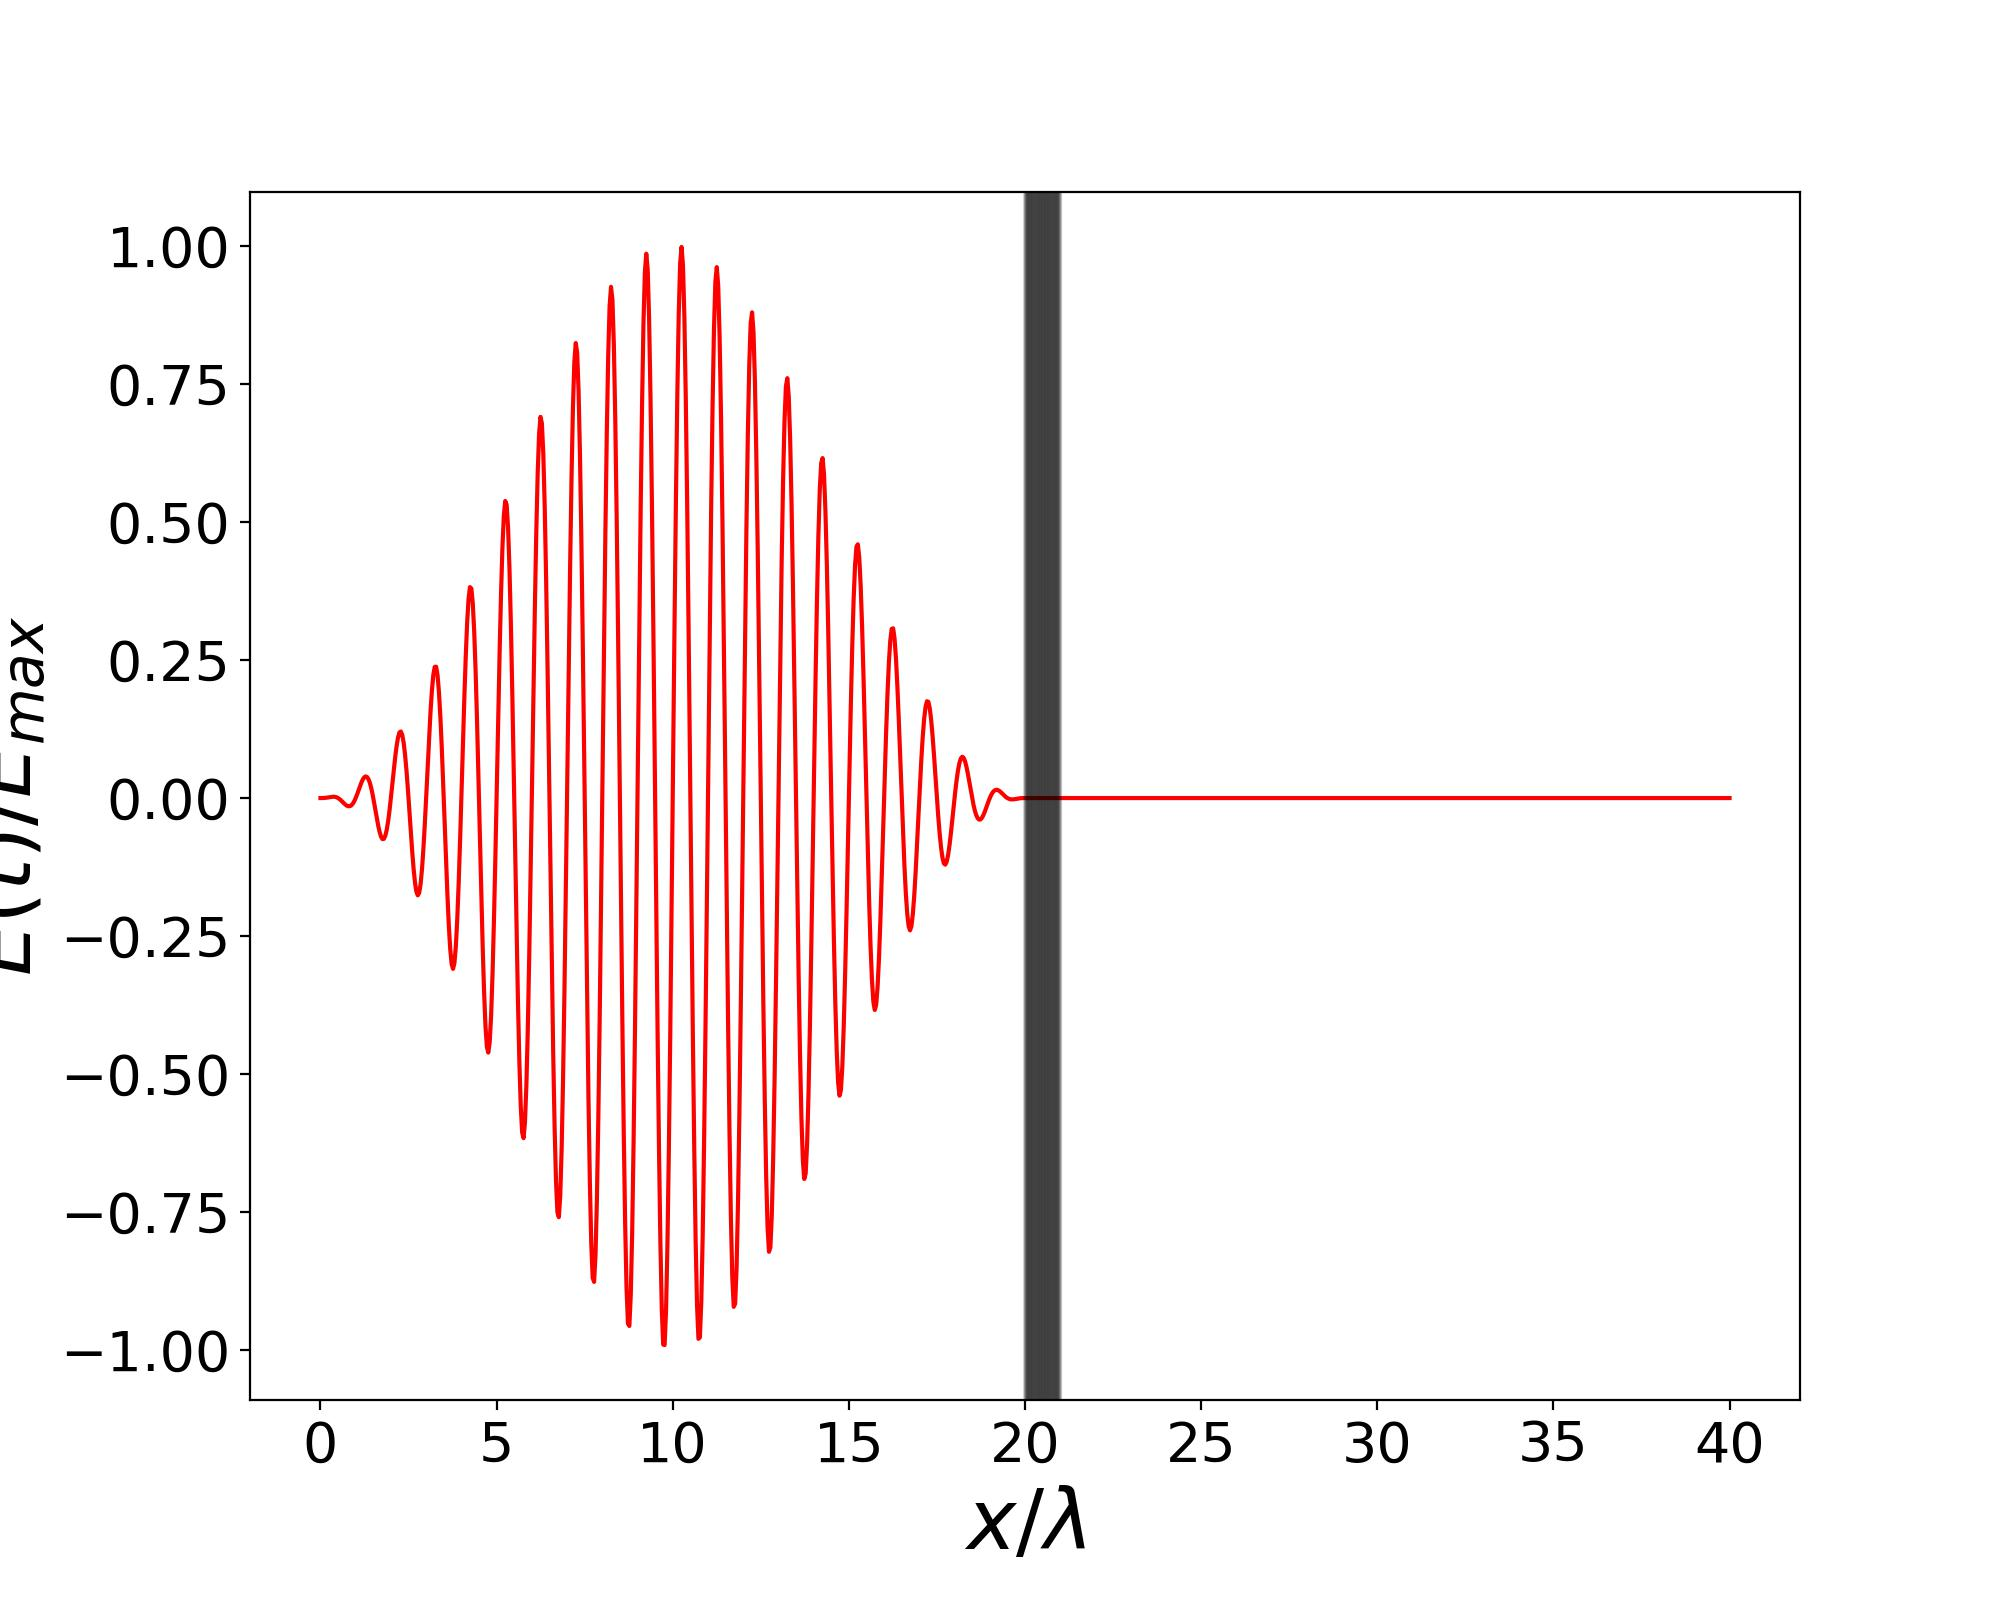
\includegraphics[width=0.9\textwidth, height=0.42\textheight]{images/field.jpg}
        % \caption{Effect of plasma density on generated harmonics}
        \label{fig:field}
    \end{minipage}
    \begin{minipage}[h]{0.48\linewidth}
        \begin{figure}
            \centering
            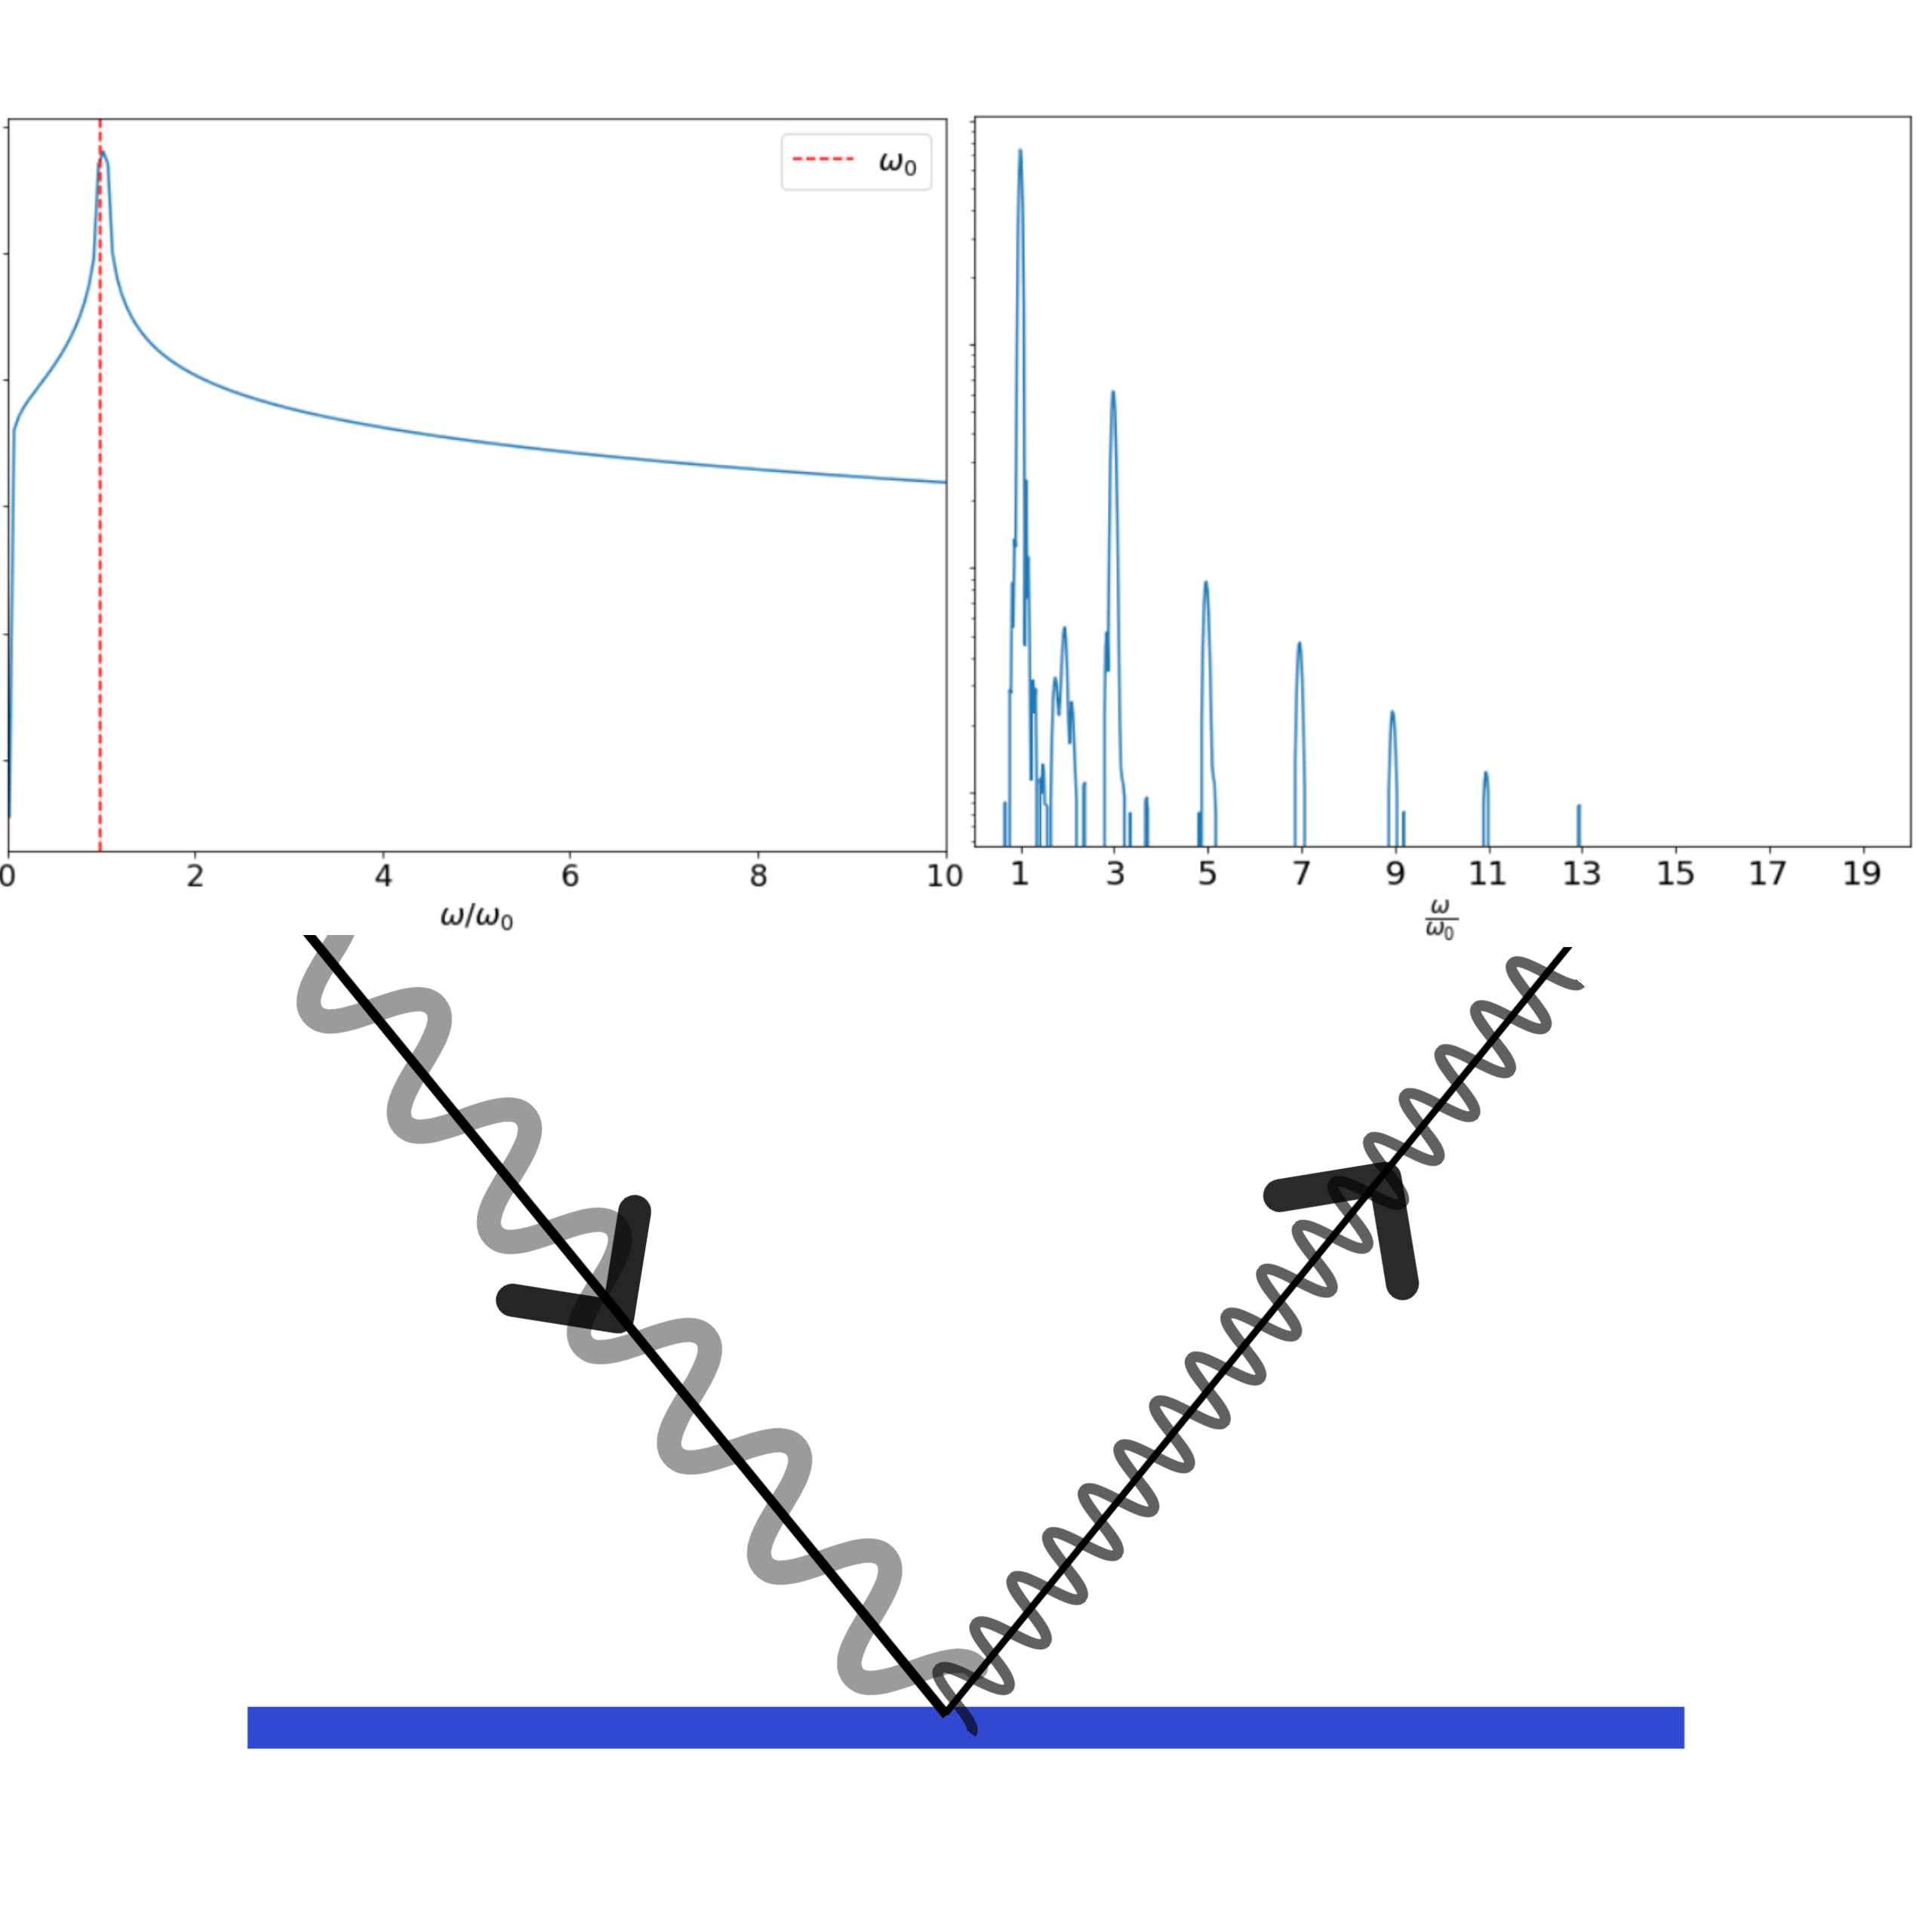
\includegraphics[width=0.9\textwidth, height=0.42\textheight]{images/harmonics.png}
            % \caption{Effect of plasma density on generated harmonics}
            \label{fig:harmonics}
        \end{figure}
        % \centering
        % 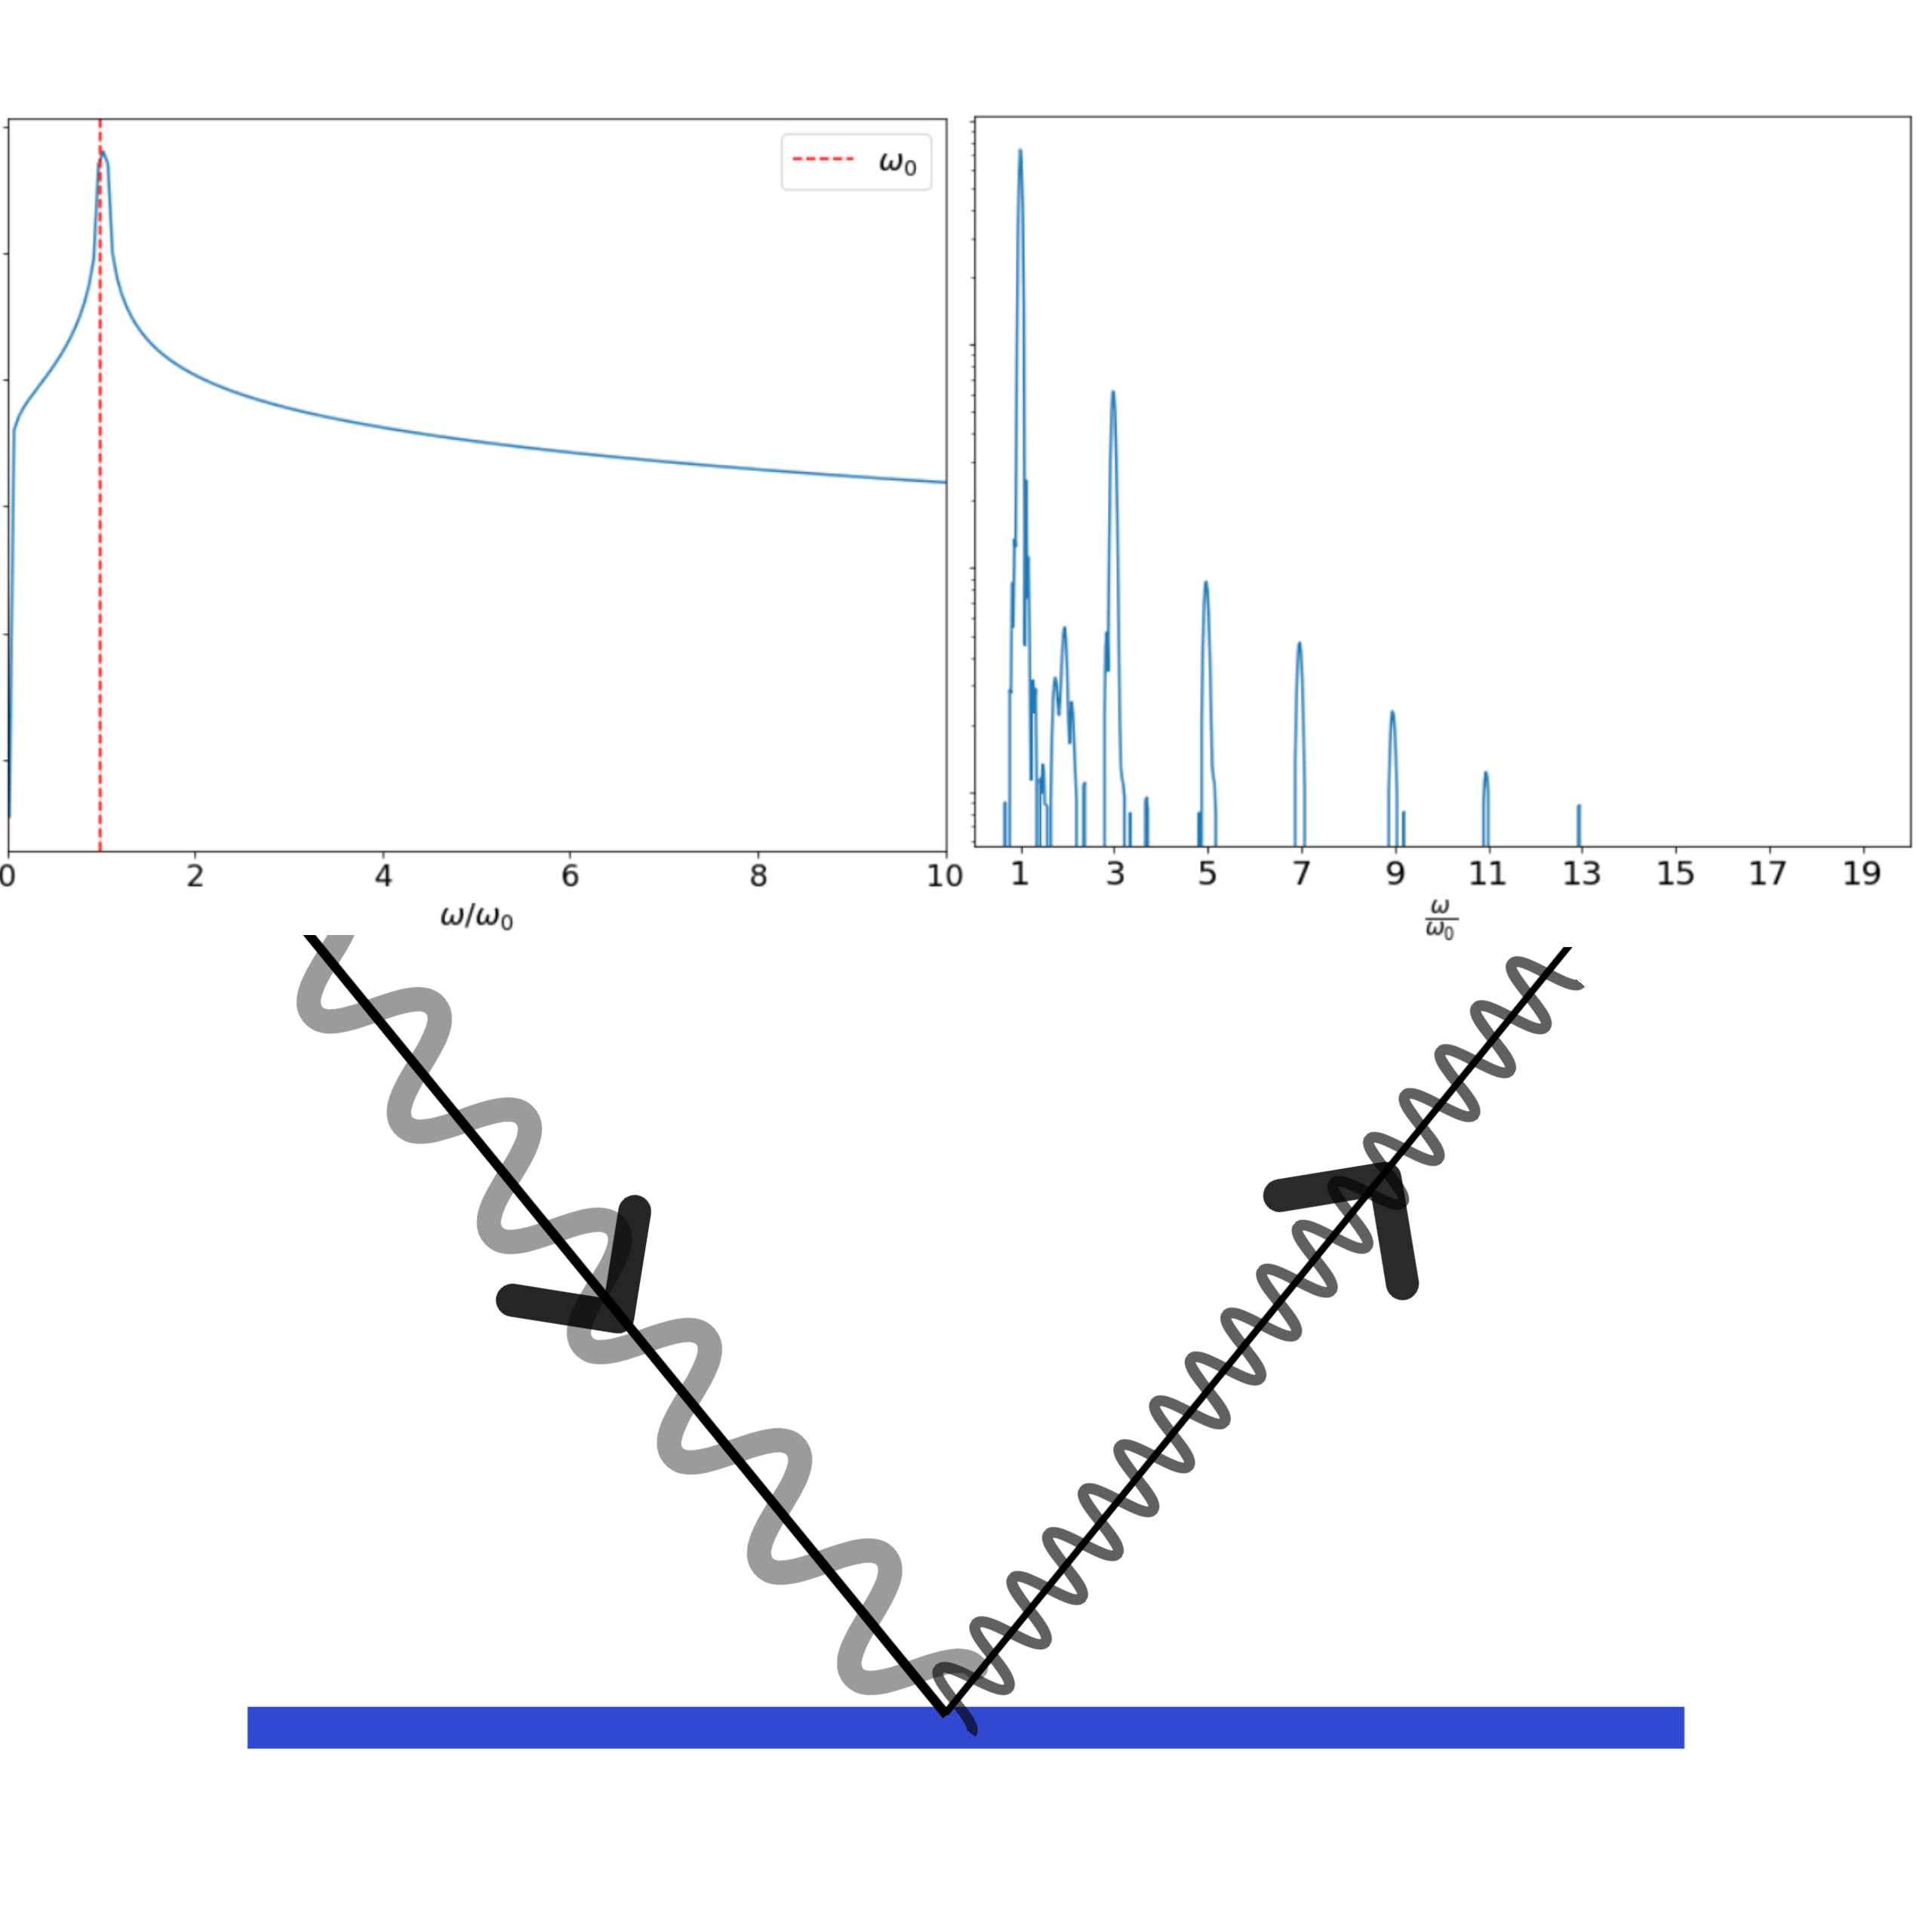
\includegraphics[width=0.7\linewidth]{images/harmonics.png}
        %     right part
    \end{minipage}
    % \footnotetext[1]{\textit{Henri Vincenti} 10.1103/physrevlett.123.105001}
    % \footnotetext[2]{\textit{Jin Woo Yoon et al} 10.1364/OPTICA.420520}
    % \footnotetext[3]{\textit{R. Lichters et al} 10 . 1063 / 1 . 871619}
\end{frame}
\begin{frame}
    \frametitle{PIC Cycle}
    \small
    The simulation uses \textit{EPOCH}\footnotemark  which implements a particle in cell algorithm.
    \begin{figure}
        \centering
        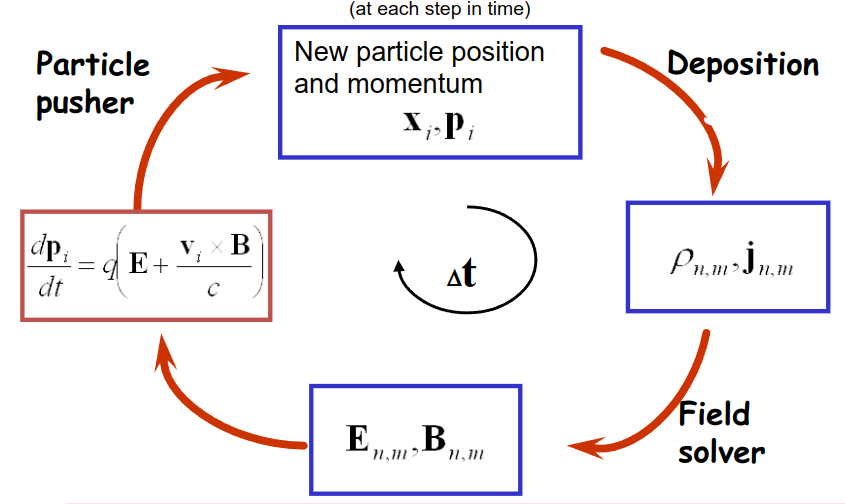
\includegraphics[width=0.9\textwidth, height=0.60\textheight]{images/PIC.png}
        \label{fig:pic}
    \end{figure}
    \begin{itemize}
        \item Interaction of laser pulse with plasma
        \item Effect of relativistic laser pulse
    \end{itemize}
    \footnotetext[4]{\textit{T D Arber et al} 10.1088/0741-
        3335/57/11/113001}
\end{frame}
\begin{frame}
    \frametitle{Simulation Details}
    \small
    We want to study the effect of various plasma and laser parameters on the generated high harmonics. We performed some simulations in 1D3V. The parameters which are constant throughout the entire experimentation are these:
    % \begin{itemize}
    %     \item The simulation box extends for $40 \lambda _l$ (from $-20 \lambda _l$ to $20 \lambda _l$), $\lambda_l = 1 \mu m$
    %     \item Number of cells is 16000 and the plasma is placed at $x=0$ and with a thickess of $\lambda_l$. There are 100 particles per cell.
    %     \item Pulse duration is  $T = 20 \tau$ and simulation is run till $T_{end} = 40 \tau$. $\tau$ is time period of laser pulse $\approx 3.3 fs$
    % \end{itemize}

    \begin{minipage}[t]{0.48\linewidth}
        % left particle
        \begin{itemize}
            \item Particles per cell: 100
            \item Number of cells: 16000
            \item Pulse duration $= 20 \tau$ ($\tau\approx 3.3 fs$)
            \item Simulation time $= 40 \tau$
            \item Wavelength $\lambda_l = 1 \mu m$
            \item Intensity of laser for $a_0 = 1$ is $I = 1.37 \times 10^{18} W/cm^2$
            \item Some parameters are varied to study their effect on the generated high harmonics.
        \end{itemize}
        % Some parameters are varied to study their effect on the generated high harmonics. These parameters and their effect on the harmonics are discussed in the next section.
    \end{minipage}
    \begin{minipage}[t]{0.48\linewidth}
        \begin{figure}
            \centering
            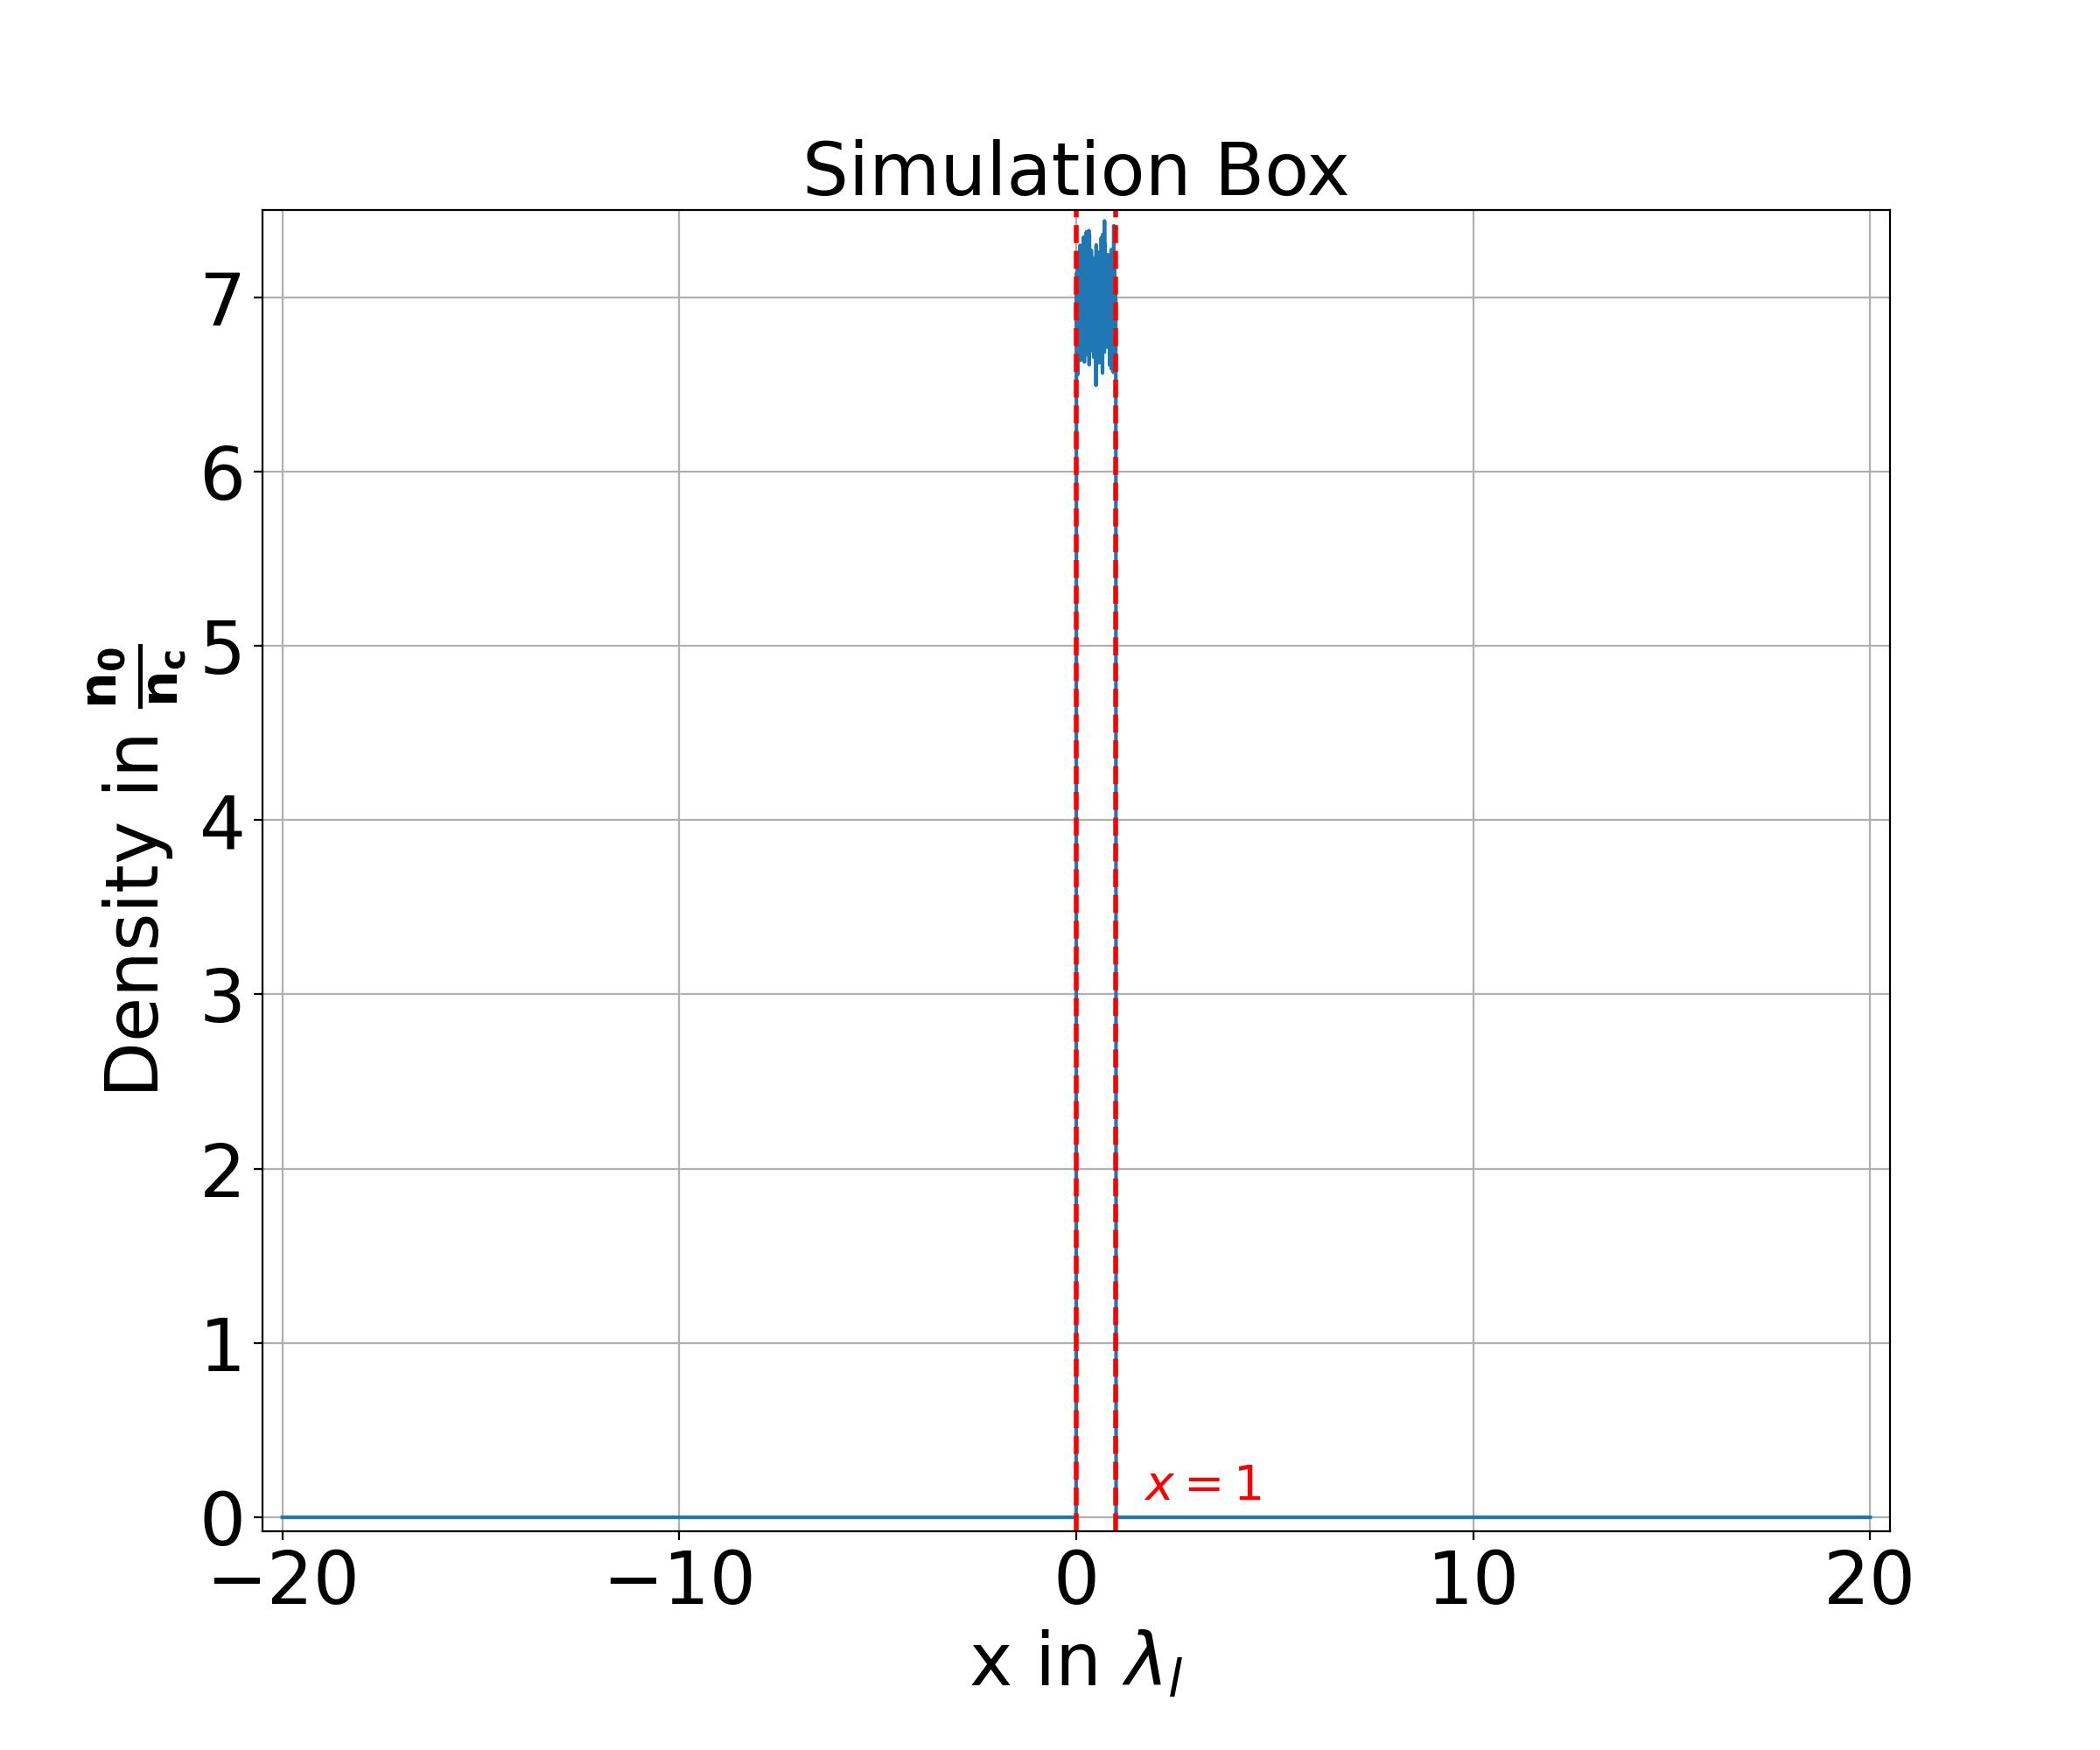
\includegraphics[width=1.0\textwidth, height=0.62\textheight]{images/plasma.jpg}
            \label{fig:plasma}
        \end{figure}
    \end{minipage}


\end{frame}

\begin{frame}
    % \frametitle{Effect of Plasma Density and Laser Intensity}
    % \Large
    \small
    % \Large
    \textbf{Effect of Laser Intensity}
    % \noindent\rule{\textwidth}{0.2pt}
    \begin{figure}
        \centering
        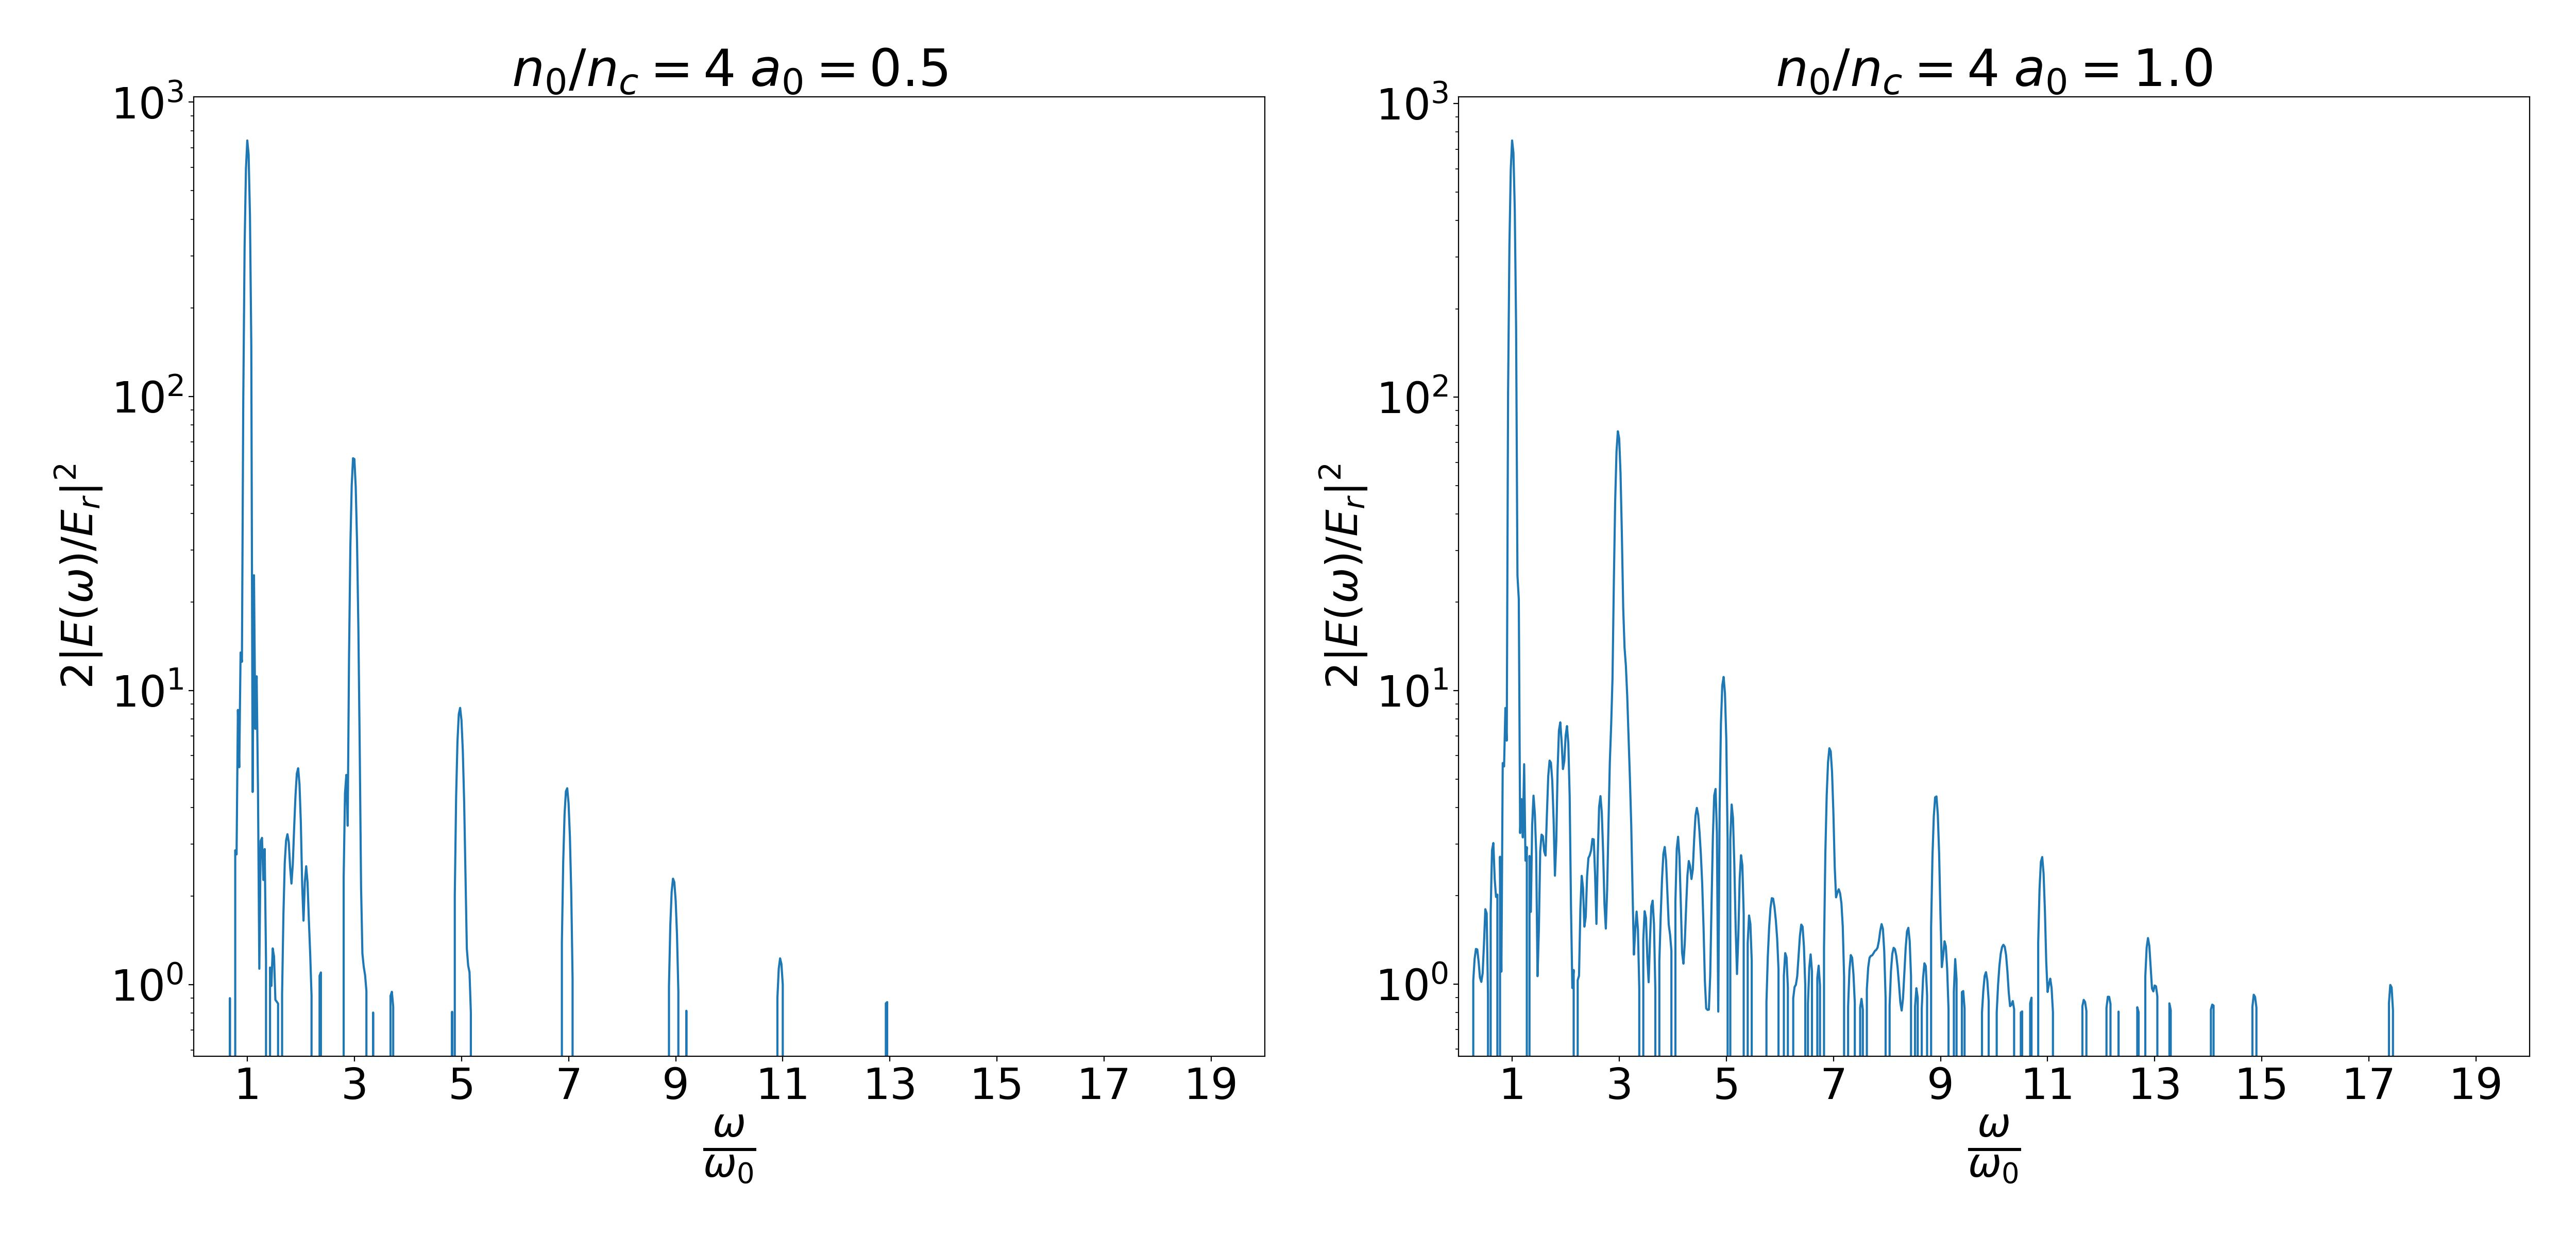
\includegraphics[width=1.0\textwidth, height=0.40\textheight]{images/intensity.jpg}
        % \caption{Effect of plasma density on generated harmonics}
        \label{fig:LaserIntensity}
    \end{figure}
    \textbf{Effect of Plasma Density}
    % \begin{minipage}[t]{0.48\linewidth}
    %     left part
    % \end{minipage}
    % \begin{minipage}[t]{0.48\linewidth}
    %     right part
    % \end{minipage}
    \begin{figure}
        \centering
        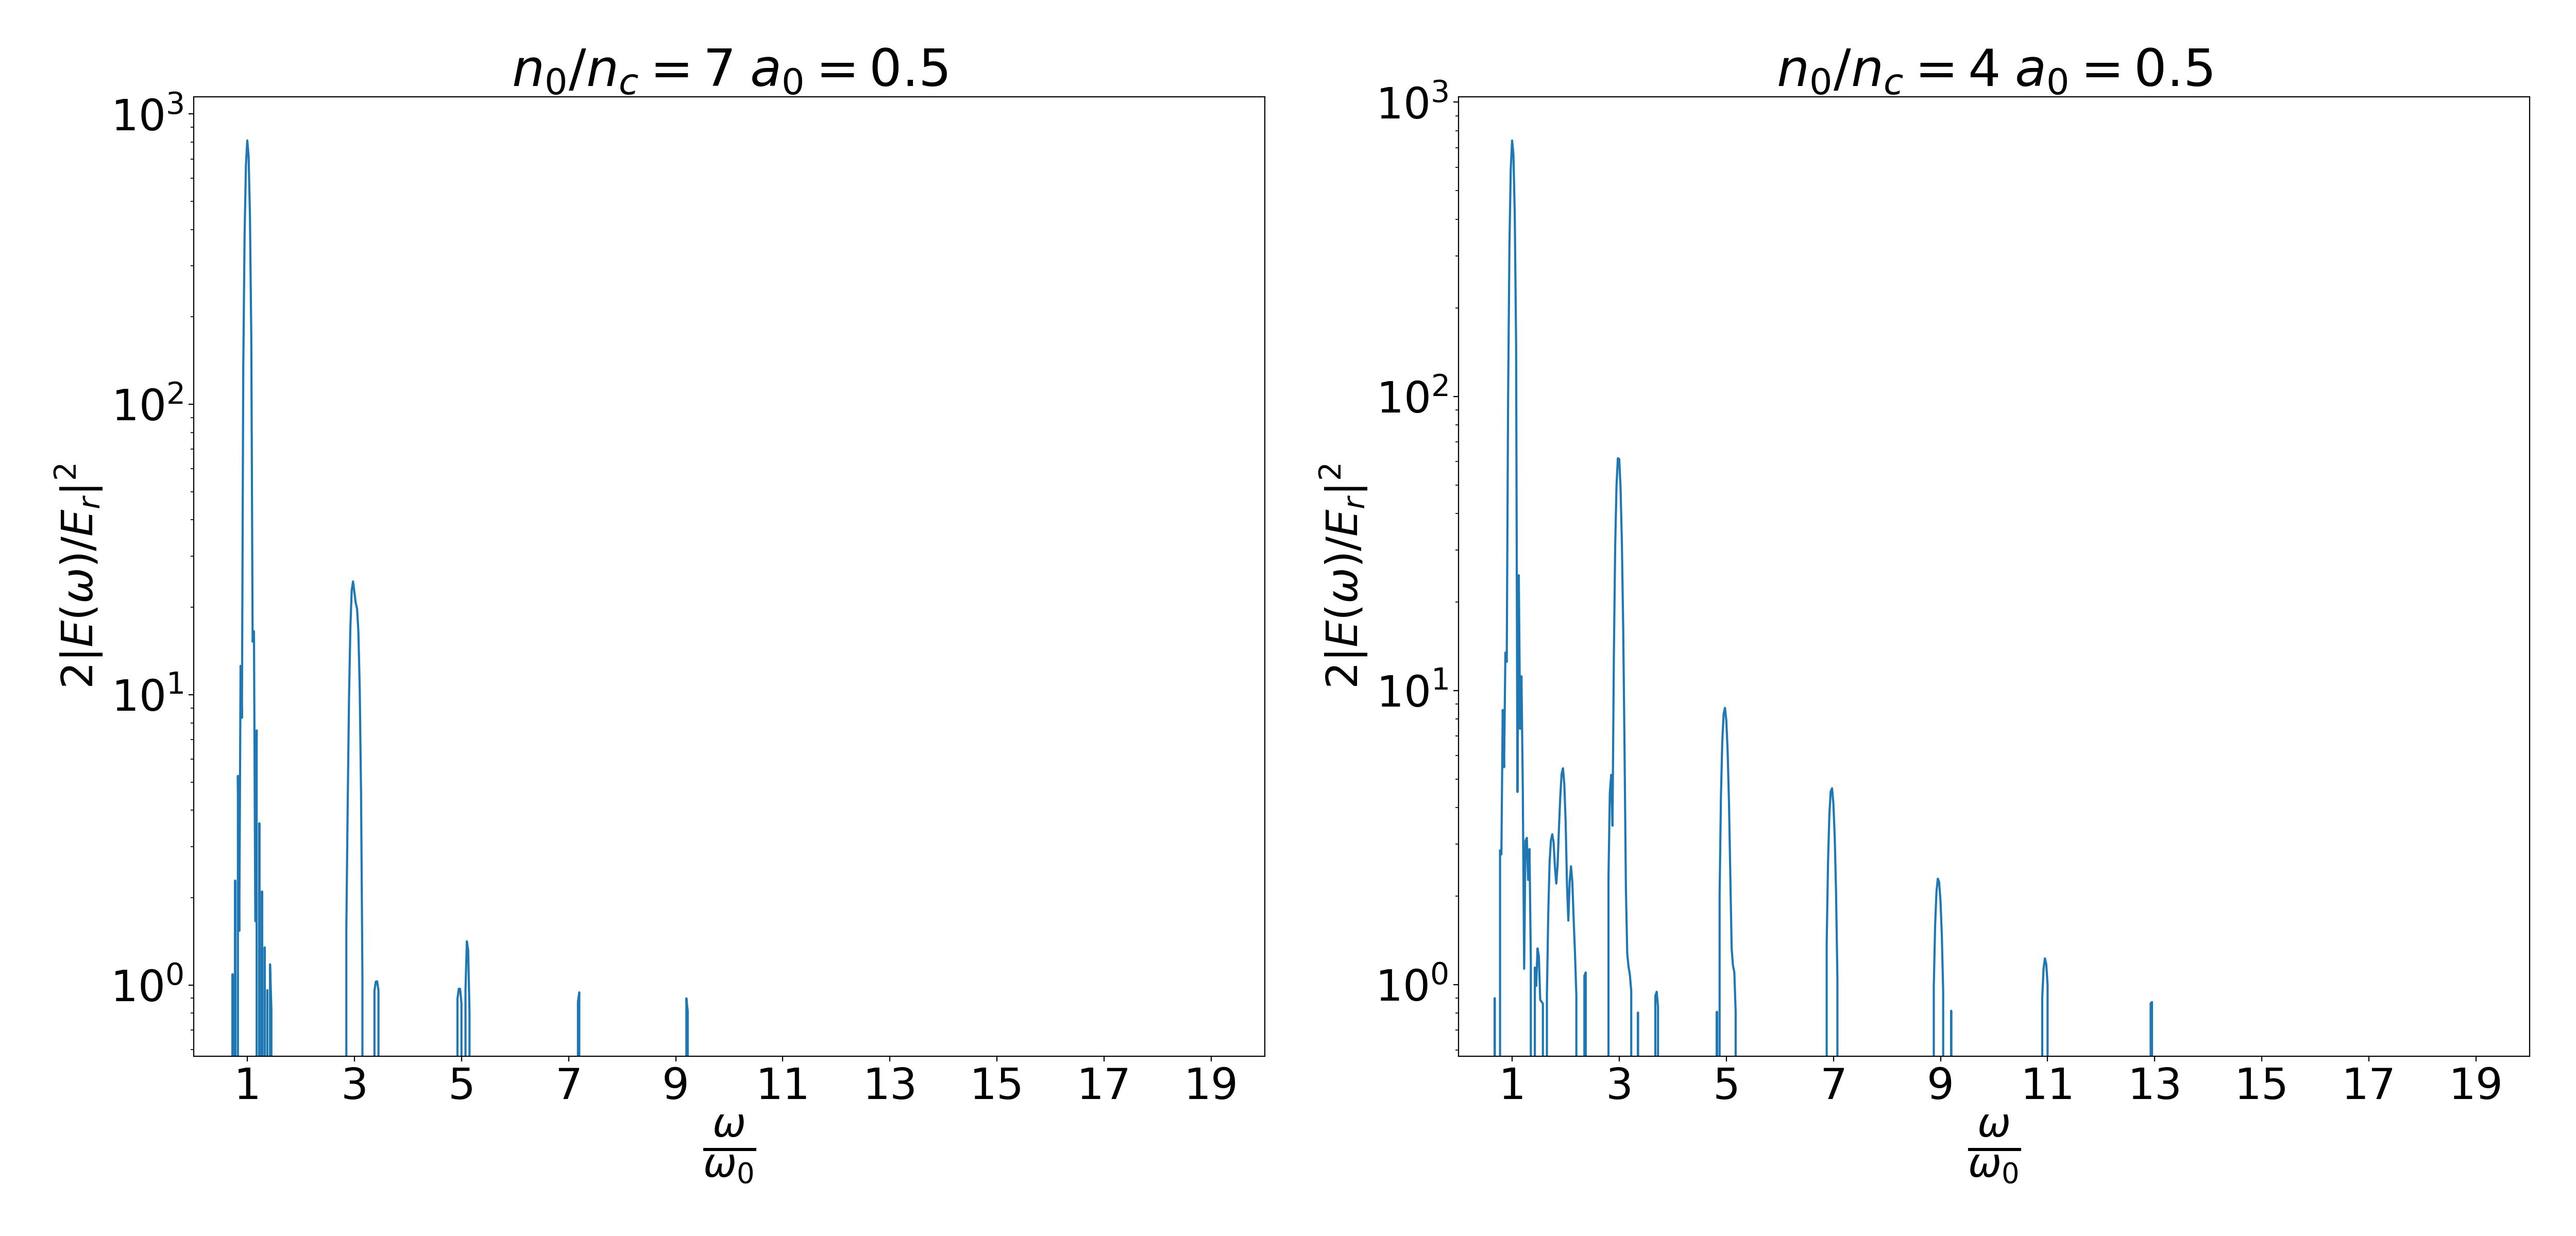
\includegraphics[width=1.0\textwidth, height=0.40\textheight]{images/density.jpg}
        % \caption{Effect of plasma density on generated harmonics}
        \label{fig:PlasmaDensity}
    \end{figure}
\end{frame}

\begin{frame}
    \frametitle{Effect of Laser Envelope}
    \tiny
    \begin{minipage}[t]{0.35\linewidth}
        1. Sine Sqaured
        \begin{equation*}\label{sin-sq-env}
            P(t)=
            \begin{cases}
                 & \sin^2(\pi t/T) \text{ for } 0 \leq t \le T \\
                 & 0         \;      \text{ otherwise }
            \end{cases}
        \end{equation*}
        2. Gaussian
        \begin{equation*}\label{gaussian-env}
            P(t)=
            \begin{cases}
                 & e^{\frac{-(t-T/2)^2}{2(0.2T)^2}} \text{ for } 0 \leq t \le T \\
                 & 0         \;      \text{ otherwise }
            \end{cases}
        \end{equation*}
        3. Triangular
        \begin{equation*}\label{triangle-env}
            P(t)= 2\times
            \begin{cases}
                 & t/T \text{ for } 0 \leq t \le T/2    \\
                 & 1-t/T \text{ for } T/2 \leq t \le T  \\
                 & 0         \;      \text{ otherwise }
            \end{cases}
        \end{equation*}
    \end{minipage}
    \begin{minipage}[t]{0.64\linewidth}
        \begin{figure}
            \centering
            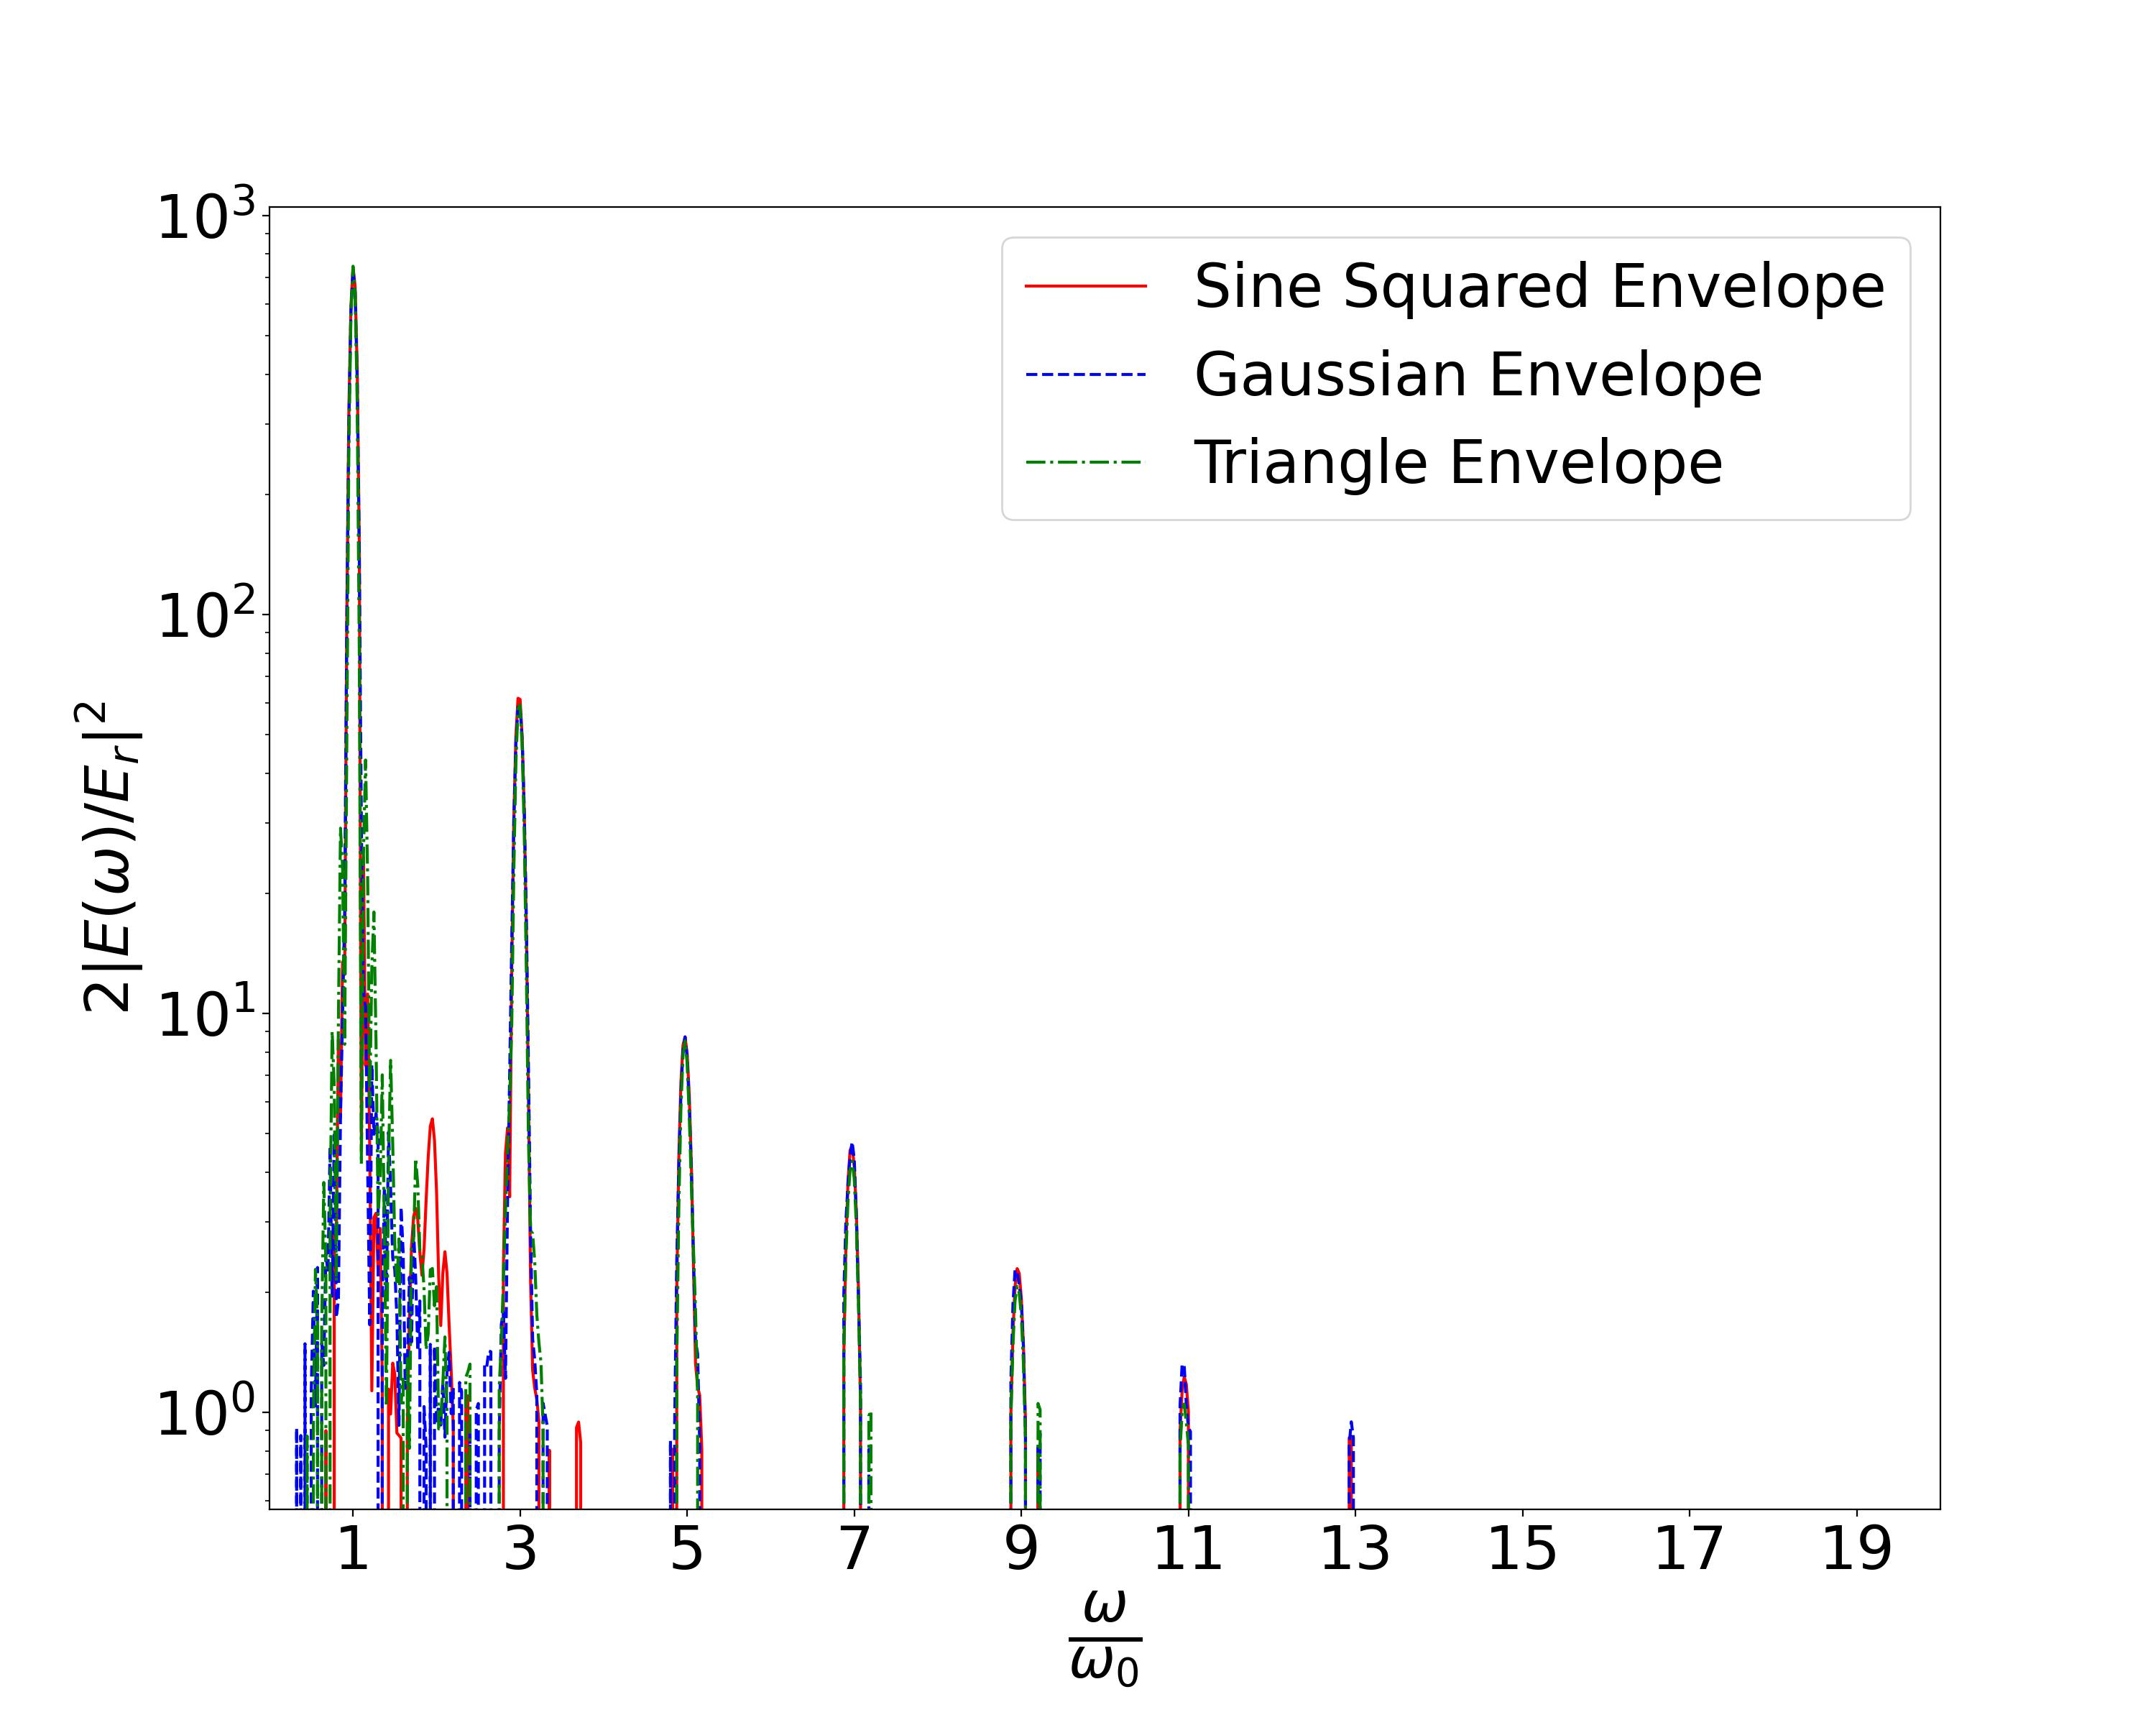
\includegraphics[width=1.0\textwidth, height=0.8\textheight]{images/env2.jpg}
            % \caption{Effect of plasma density on generated harmonics}
            \label{fig:LaserEnv}
        \end{figure}
    \end{minipage}

\end{frame}

\begin{frame}
    \frametitle{Effect of Pulse Length}
    \begin{figure}
        \centering
        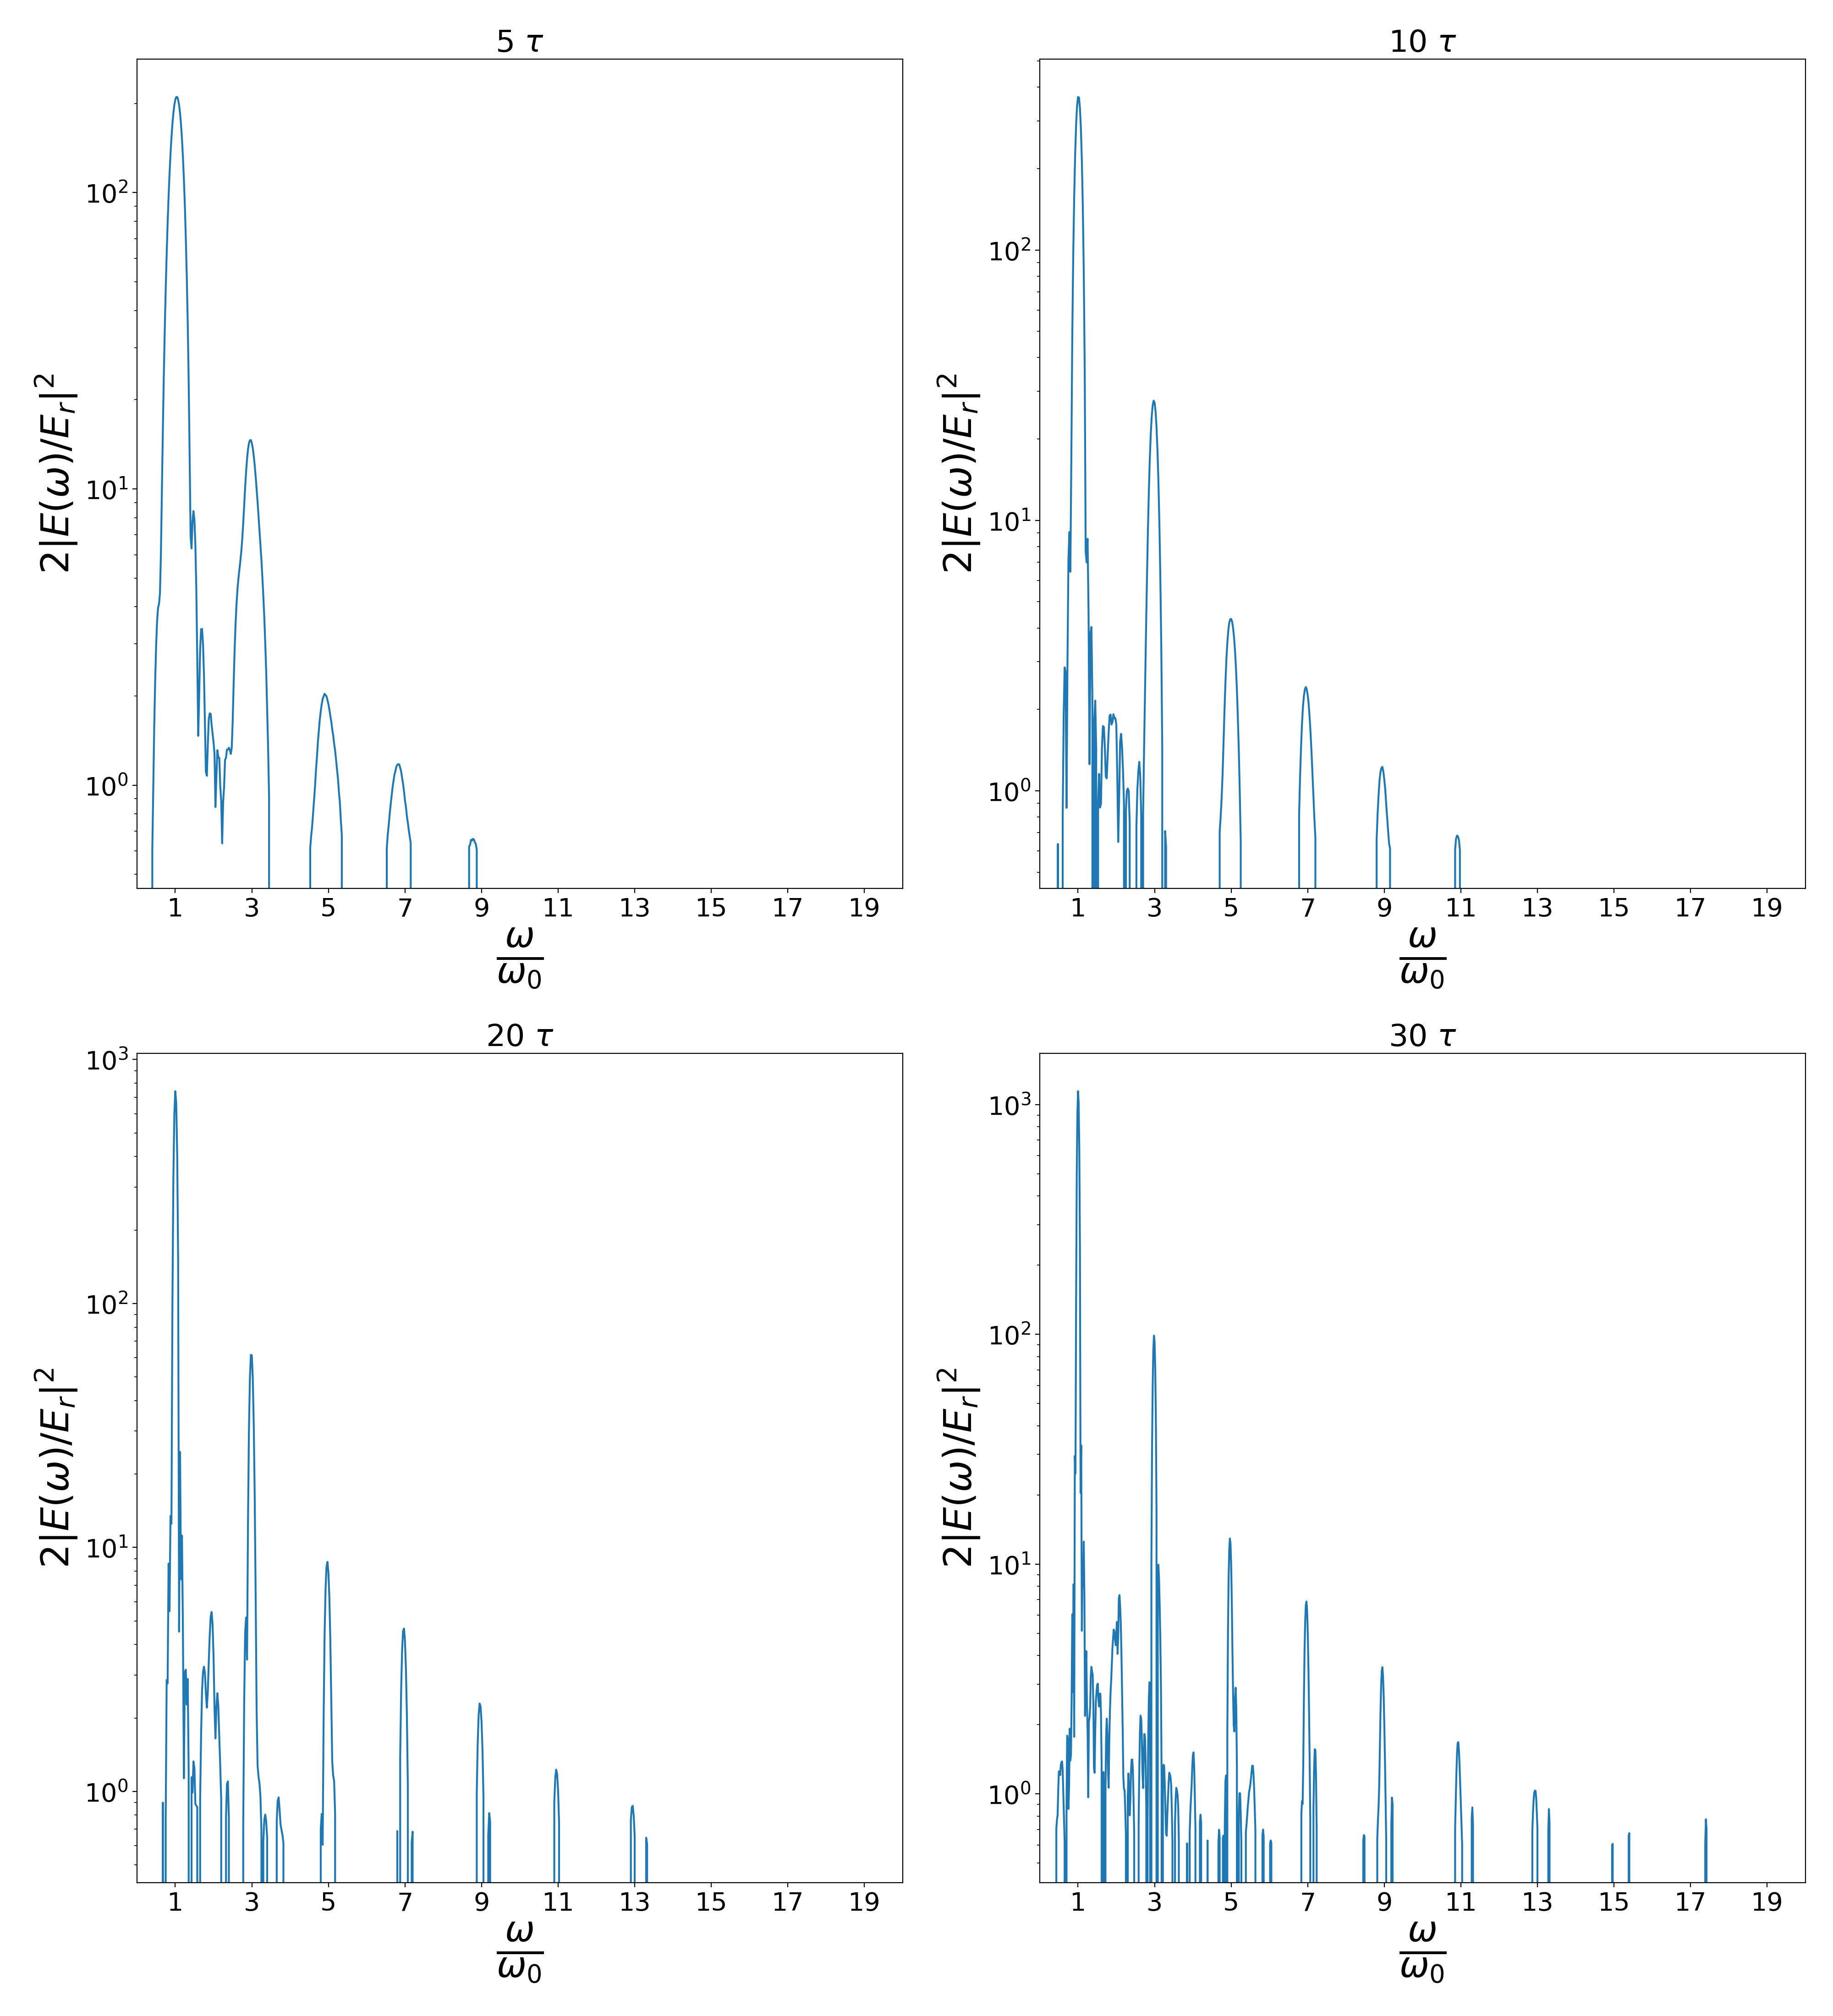
\includegraphics[width=1.0\textwidth, height=0.8\textheight]{images/pulse.jpg}
        % \caption{Effect of plasma density on generated harmonics}
        \label{fig:LaserPulsev}
    \end{figure}
\end{frame}
\begin{frame}
    \frametitle{Effect of Laser Intensity on Electron Oscillations}
    \begin{figure}
        \centering
        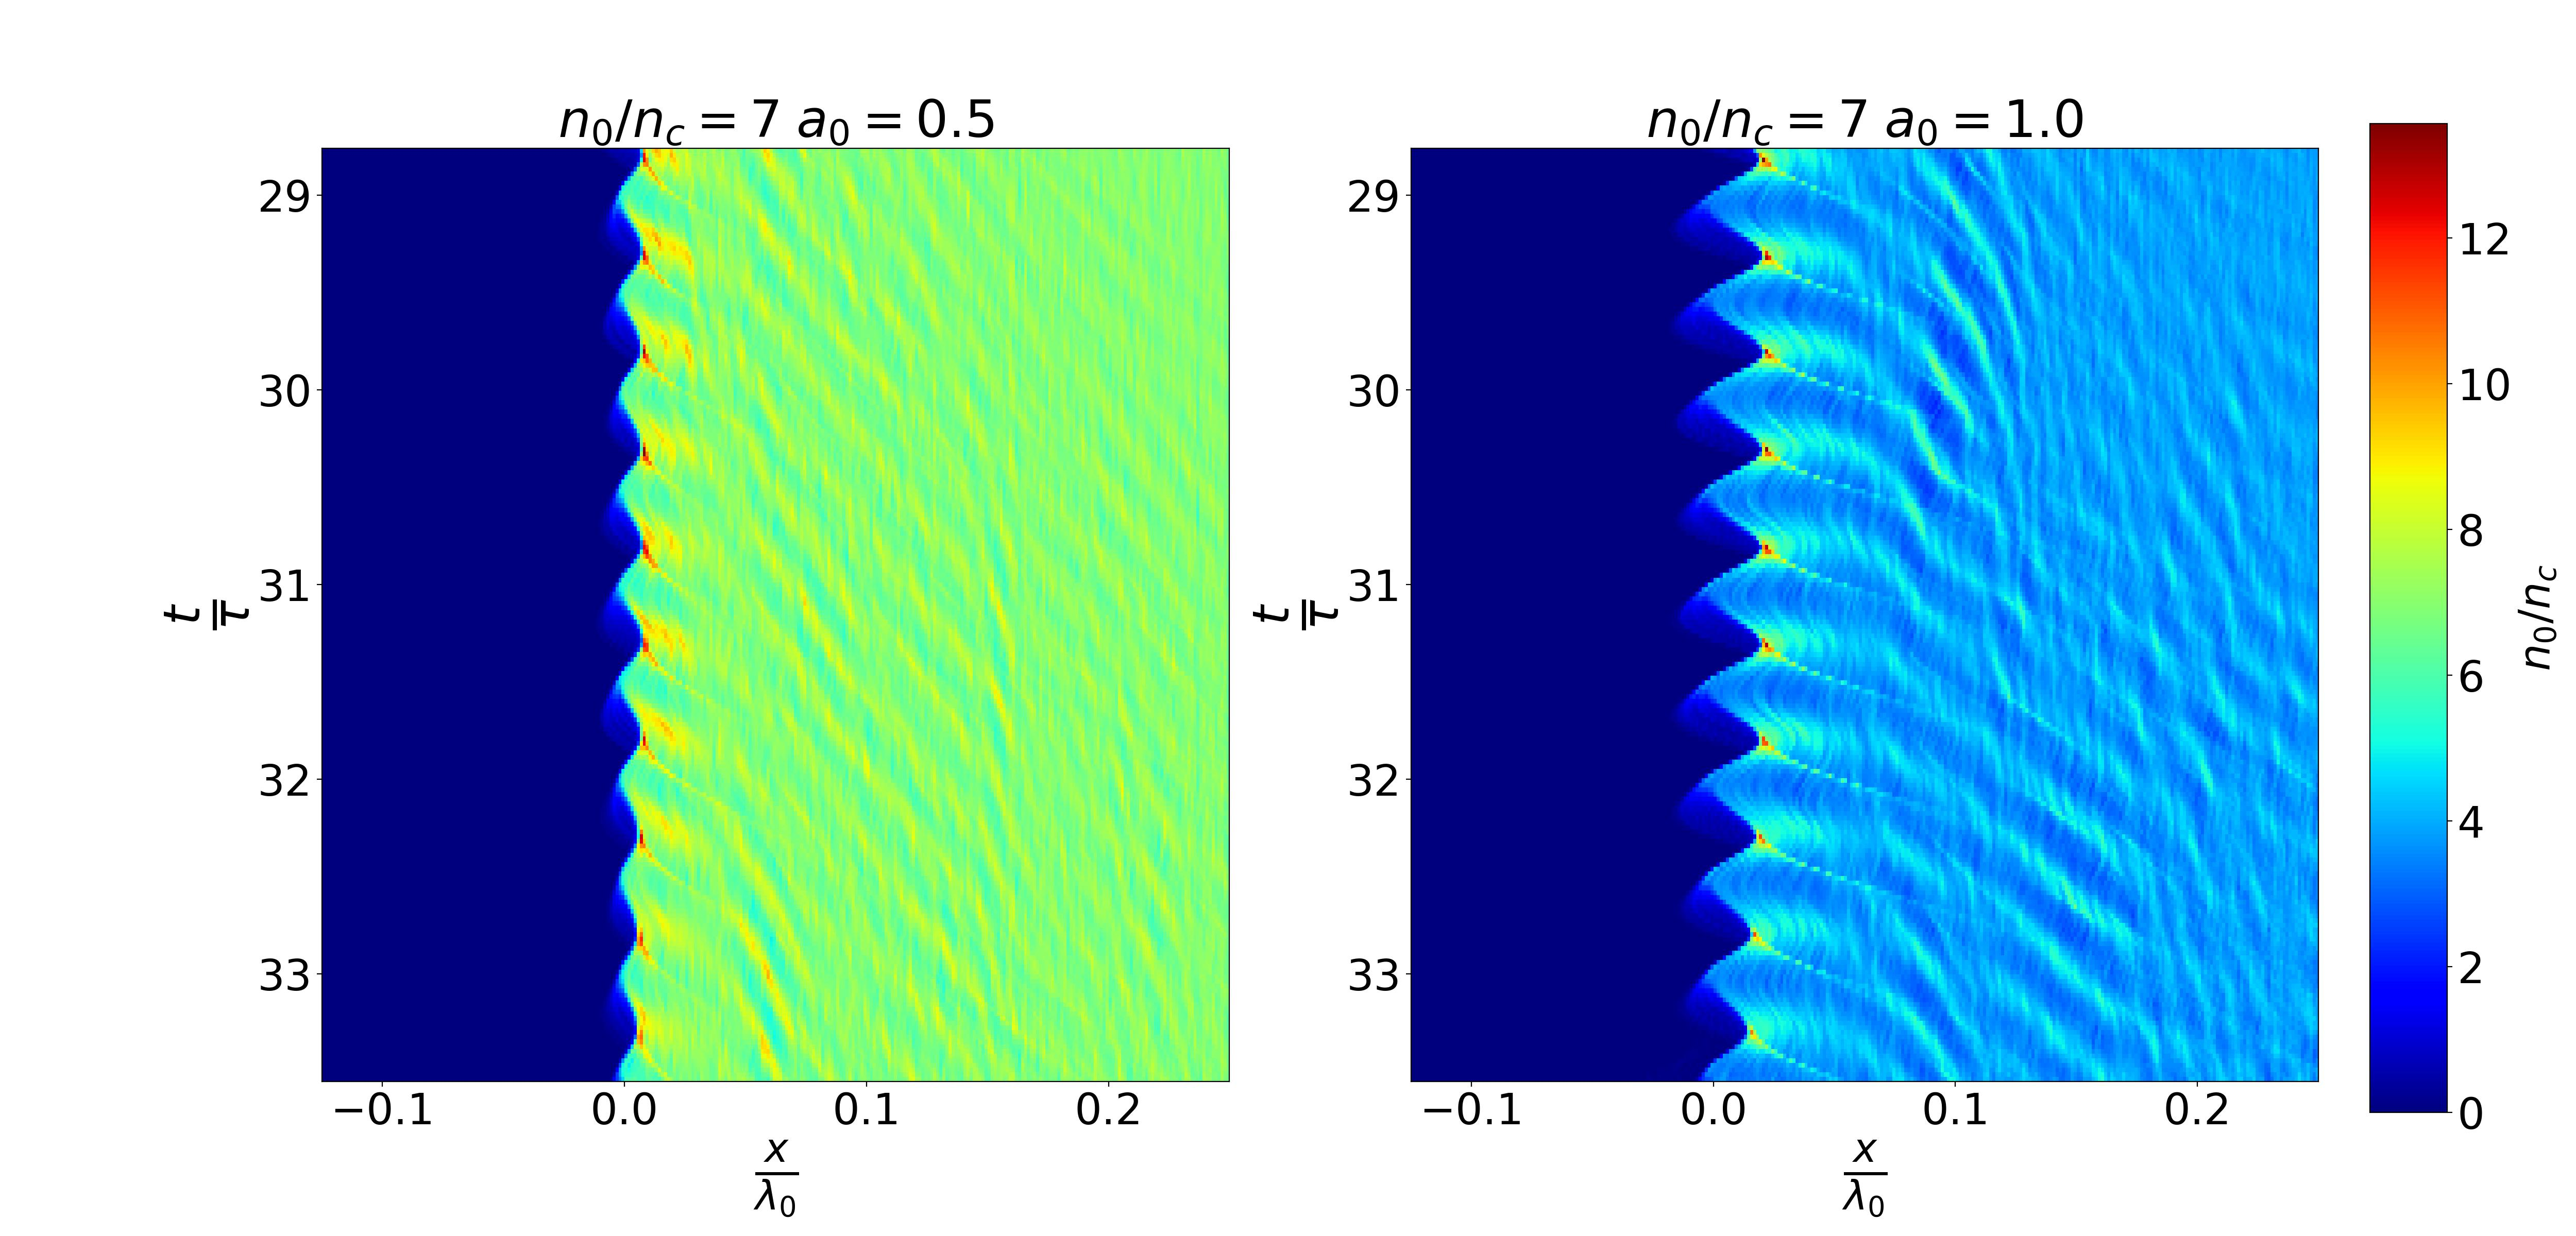
\includegraphics[width=1.0\textwidth, height=0.8\textheight]{images/oscillation1.jpg}
        % \caption{Effect of plasma density on generated harmonics}
        \label{fig:Oscillations1}
    \end{figure}
\end{frame}

\begin{frame}
    \frametitle{Frequency of the Oscillations}
    \begin{figure}
        \centering
        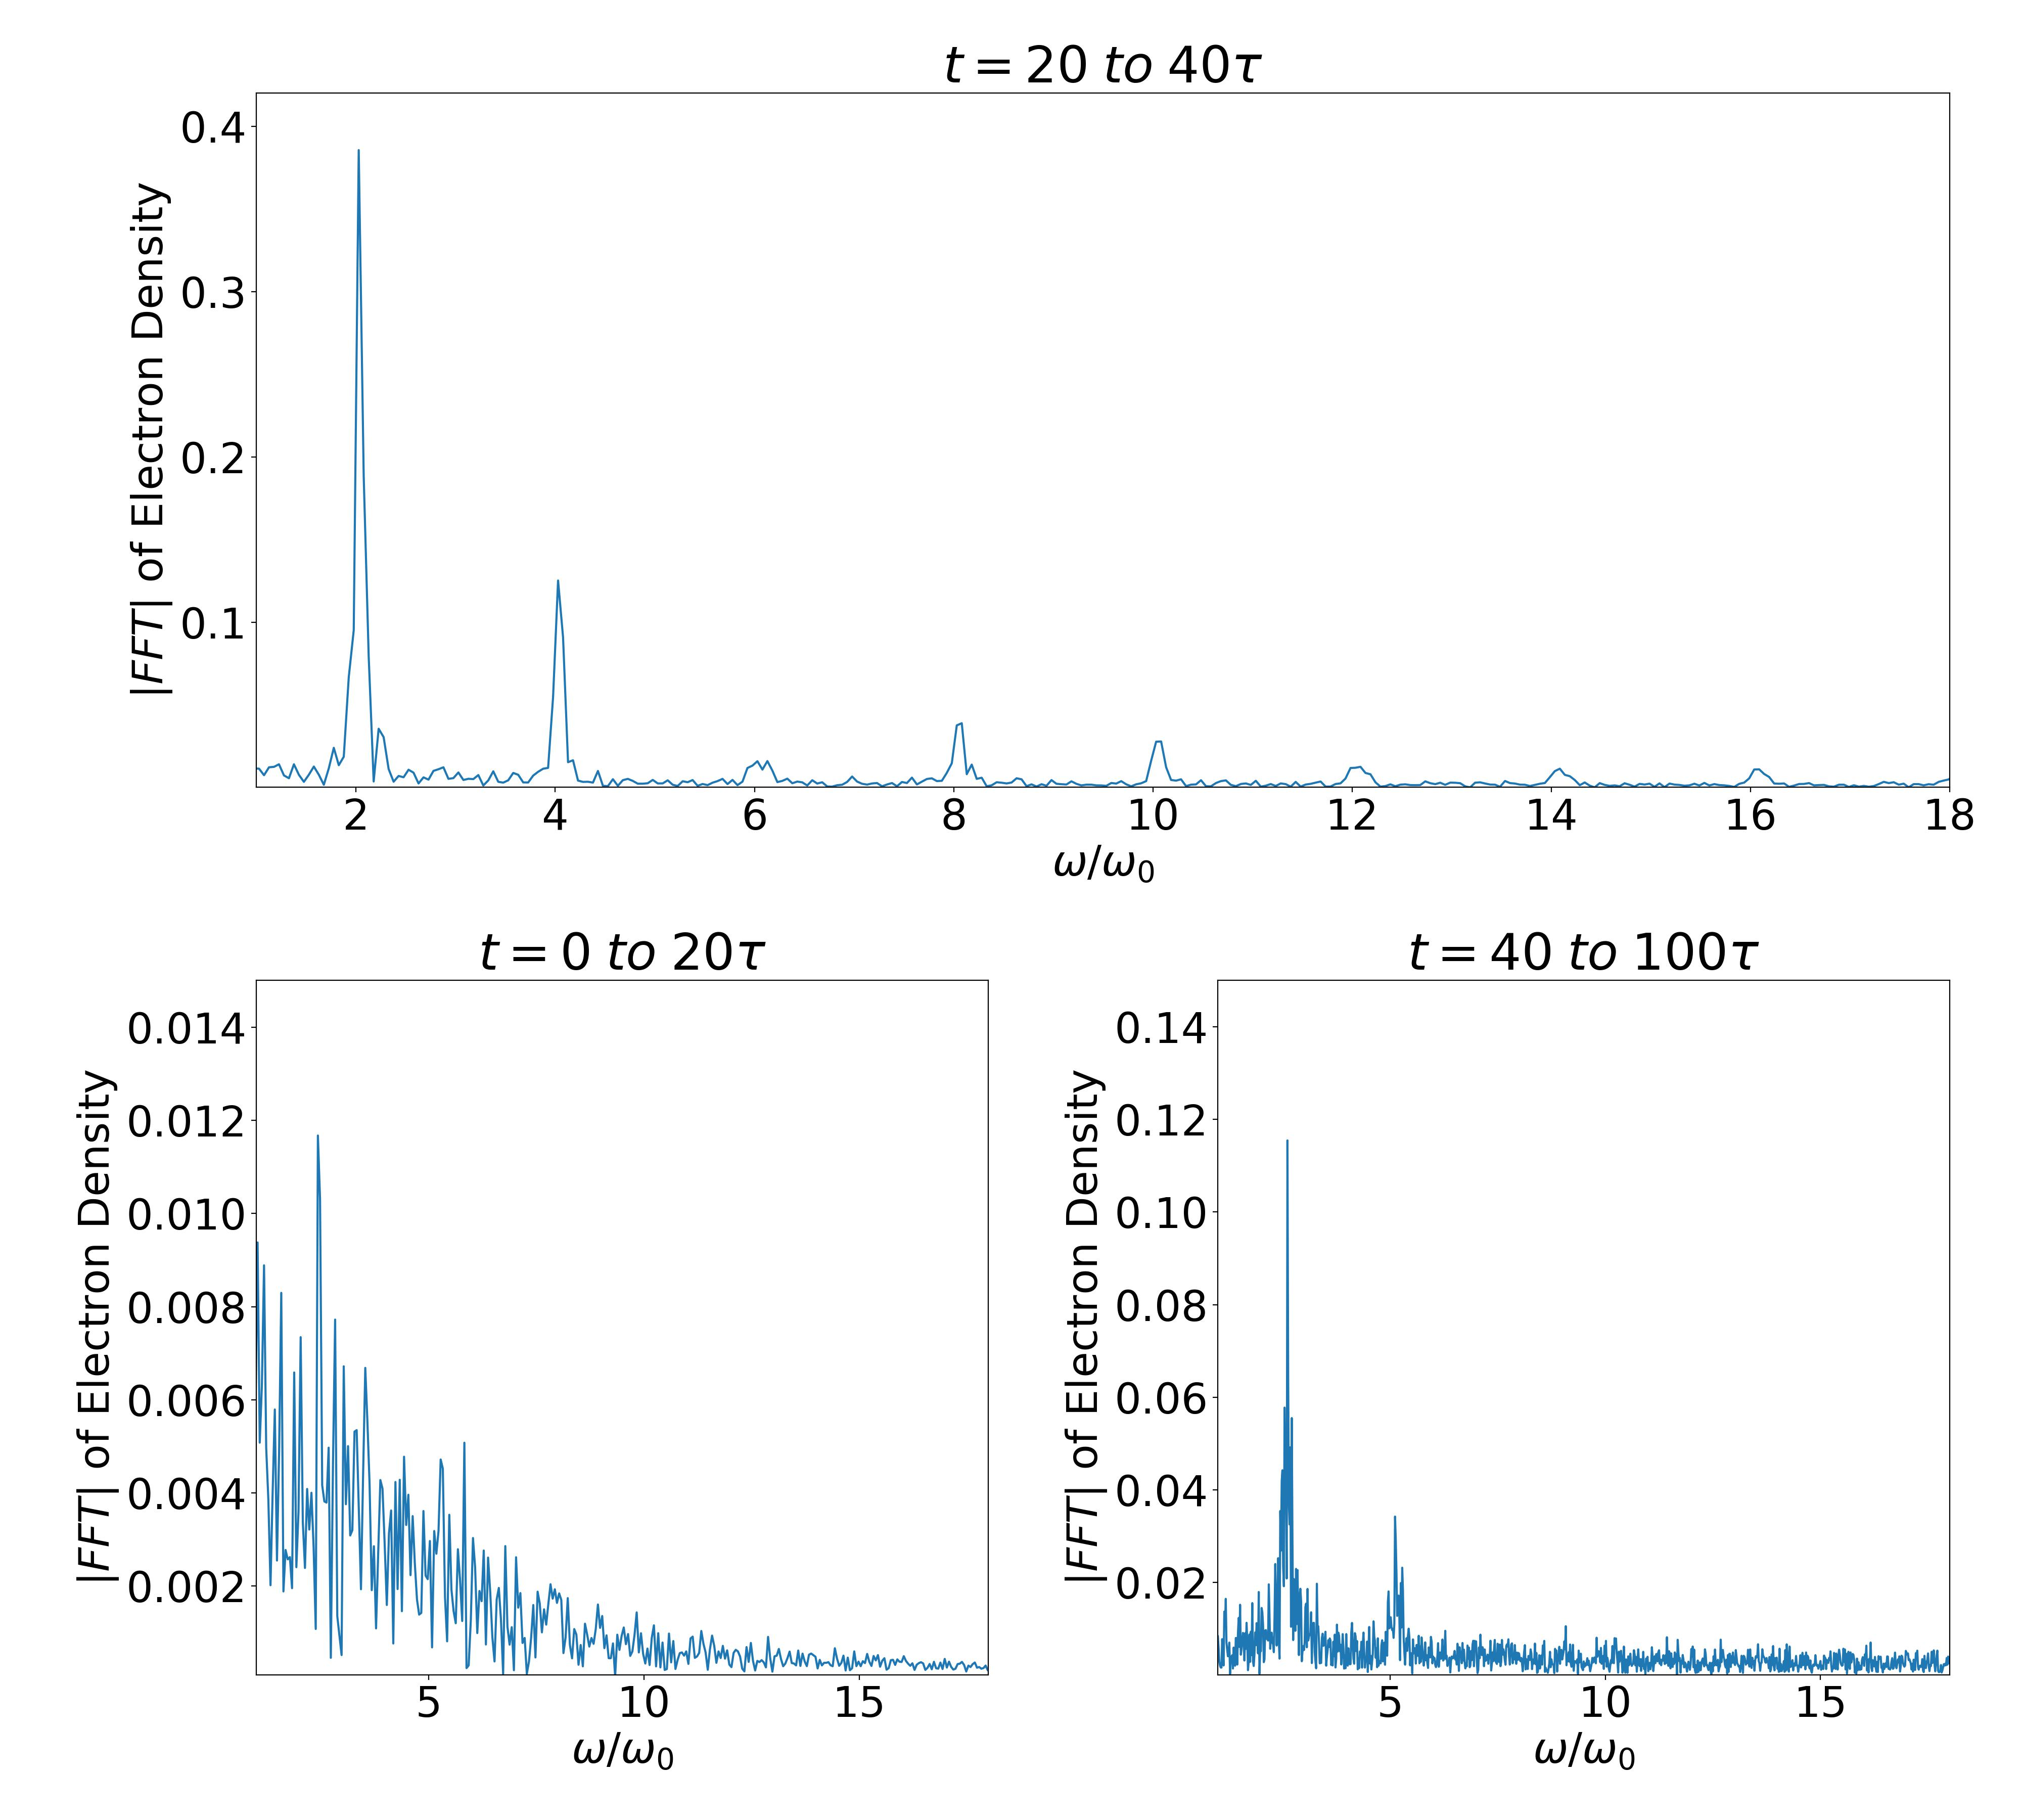
\includegraphics[width=0.8\textwidth, height=0.8\textheight]{images/oscillation2.jpg}
        % \caption{Effect of plasma density on generated harmonics}
        \label{fig:Oscillations2}
    \end{figure}
\end{frame}
\begin{frame}
    \frametitle{Current Status and Future Plan of Work}
    \textbf{Current Status}
    \begin{itemize}
        \item Only odd harmonics are generated
        \item A resonance at $n_0/n_c=4$ is also observed
              % \item No effect of density. Though a resonance at $n_0/n_c=4$ is observed
        \item Increasing intensity and pulse duration increases number of harmonics
        \item No effect of the envelopes
        \item Even harmonics are generated in electron oscillations
              % \item We have also observed the oscillations of electrons in the plasma.
              % \item We are currently working on the generation of high harmonics in the range of 50-100 nm.
              % \item We are also working on the generation of high harmonics in the presence of a magnetic field.
    \end{itemize}
    % \rule[h]
    % \\
    % \par\noindent\rule{\textwidth}{0.4pt}
    \textbf{Future Plan of Work}
    \begin{itemize}
        \item Effect of plasma density
        \item Oblique incidence
        \item Some more envelopes (Supergaussian, Laguere-Gaussian, etc.)
        \item Polarization
    \end{itemize}
    % The interaction of high intensity laser pulse with overdense plasma is investigated. During this, odd harmonics of the incident laser pulse is generated and the effect of variuos laser and plasma parameters on the hormonic generation is studied. Future plan of work is to study about the effects of some more parameters on the harmonics generation escpecially the effect of oblique incidence and different polarization of the laser pulse.
\end{frame}

% \begin{frame}
%     % \AtNextBibliography{\small}
%     % \printbibliography
% \end{frame}
\end{document}